%%
%  ******************************************************************************
%  * #file    Szablon_raportu_EN_Latex.tex
%  * #author  Adrian Wójcik   adrian.wojcik(at)put.poznan.pl
%  *          
%  * #commit  Patryk Kościk   koscikpatryk(at)gmail.com
%  *          Modified the template for Projekt przejsciowy purposes          
%  *          
%  *
%  * #commit  Patryk Kościk   koscikpatryk(at)gmail.com
%  *          Zupełnie przewrócono na łeb formatke po taktycznym wyjasnieniu          
%  *          
%  * #version 1.1
%  * #date    09-Mar-2022
%  * #brief   PROJPRZEJ
%  *
%  ******************************************************************************
%%  
\documentclass[11pt, a4paper]{article}

\usepackage{SM_template}

% Wypełnijcie te dyrektywy zgodnie z waszym tematem
%
% \lab      -> NAZWA CZUJNIKA,          np.: 'DHT22'
% \comment  -> Króciutki opis co to,    np.: 'Cyfrowy czujnik temperatury'
% \author   -> Autor dokumentu          np.: Patryk Kościk
%
% Pamiętajcie o zmianie ścieżki w \addbibresourcue (!)

\lab{Moduł KY-024}
\comment{Analogowo/cyfrowy czujnik halla}
\author{Jakub Grzesiak}
\addbibresource{bib/KY-024.bib}

%
% Początek dokumentu
%
\begin{document}

%
% Strona tytułowa
%
\mainpage{KY-024/zdj_modulu/hall_sens_final.jpg}
\newpage

\section*{Opis elementu}
Czujnik halla KY-024 to analogowo-cyfrowy sensor zbudowany z: dwóch diod LED - LD1 jest odpowiedzialna za sygnalizowanie zasilania całego układu a LD2 za sygnalizowanie wykrycia pola magnetycznego, potencjometru do regulacji czułości układu, 6 rezystorów, komparatora LM393 złożonego z dwóch wzmacniaczy operacyjnych i wysuniętego poza płytkę PCB liniowego czujnika Halla 49E. Cały układ bazuje na zjawisku magnetyzmu i pola magnetycznego, które przechodzi w danym kierunku przez sensor 49E. Czujniki tego typu znajdują zastosowanie w takich elementach jak: enkodery obrotowe, mierniki cęgowe, mangetyczne czujniki zbliżeniowe czy czujniki pozycji wału w silnikach elektrycznych.


%%%%%%%%%%%%%%%%%%%%%%%%%  TWO IMAGES SIDE BY SIDE  %%%%%%%%%%%%%%%%%%%%%%%%%%%%%
\vspace{0.25cm}
\begin{figure}[h]
\centering
%%%%%%%%%%%%%%%%%%%%%%%%%%%%%%%%%%%%%%%%%%%%%%%%%%%%%%%%%%%%%%%%%%%%%%%%%%%%%%%%%
\begin{subfigure}{.47\textwidth}
\centering
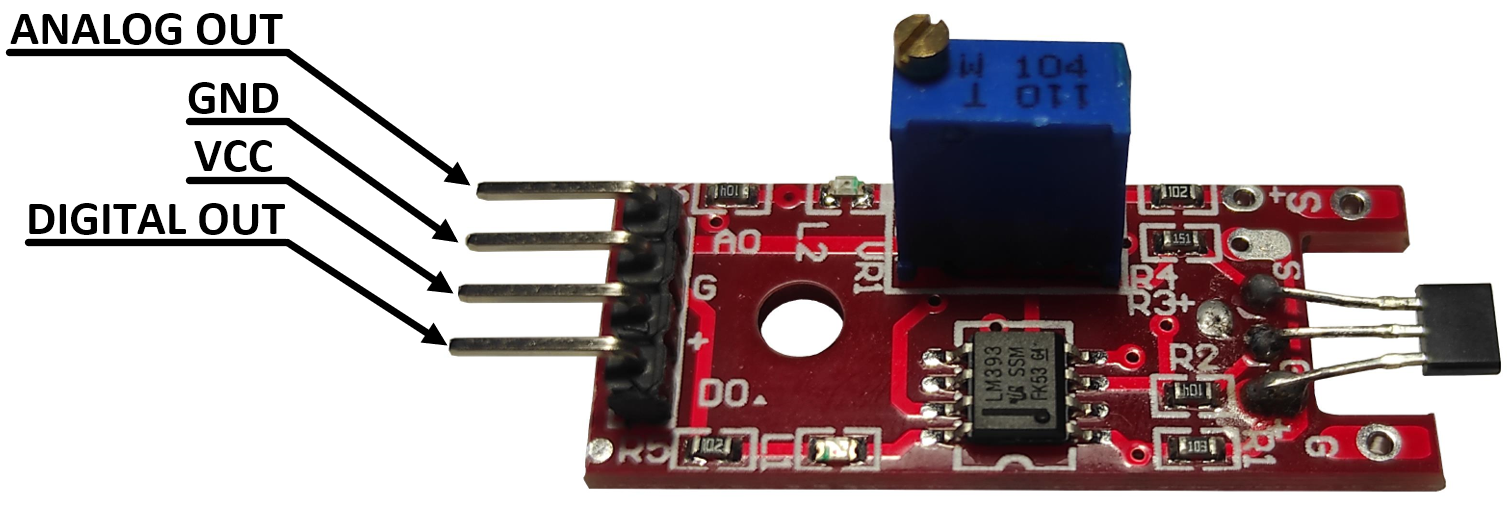
\includegraphics[width=1.1\linewidth]{fig/KY-024/zdj_modulu/pinout.png}
\caption{Fizyczna budowa czujnika wraz z pinoutem}
\label{fig:_zdjecie_elementu}
\end{subfigure}%
%%%%%%%%%%%%%%%%%%%%%%%%%%%%%%%%%%%%%%%%%%%%%%%%%%%%%%%%%%%%%%%%%%%%%%%%%%%%%%%%%
\begin{subfigure}{.6\textwidth}
\centering
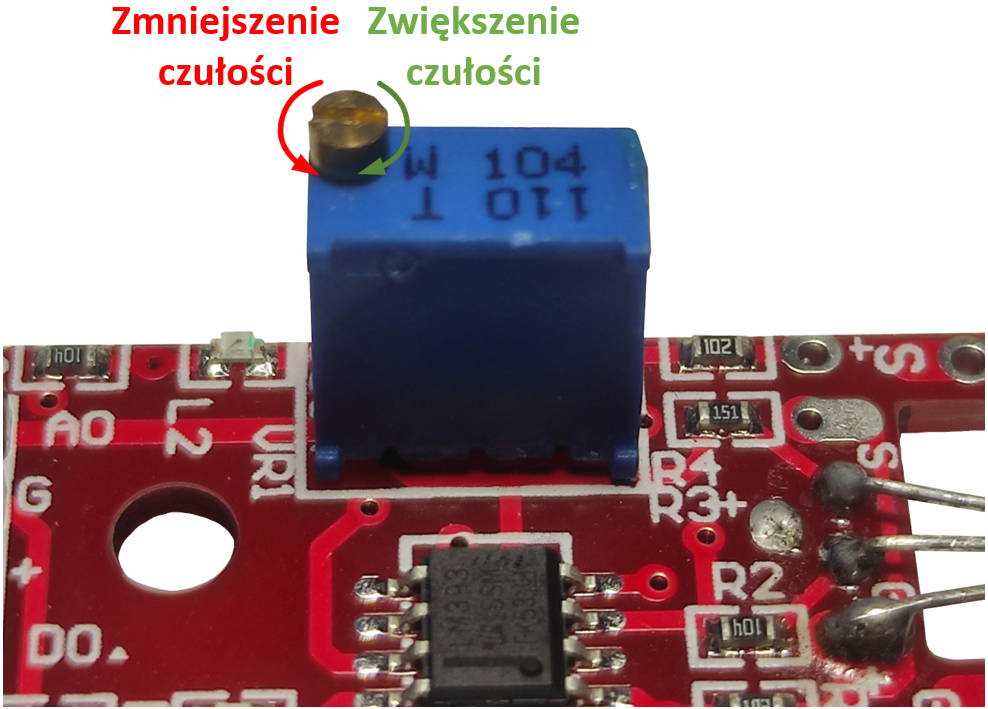
\includegraphics[width=.6\linewidth]{fig/KY-024/zdj_modulu/sensitivity.png}
\caption{Dostosowywanie czułości działania czujnika}
\label{fig:_zasada_dzialania_czulosc}
\end{subfigure}
%%%%%%%%%%%%%%%%%%%%%%%%%%%%%%%%%%%%%%%%%%%%%%%%%%%%%%%%%%%%%%%%%%%%%%%%%%%%%%%%%
% \caption{PODPIS}
\label{fig:element}
\end{figure}
\vspace{0.25cm}
%%%%%%%%%%%%%%%%%%%%%%%%%  TWO IMAGES SIDE BY SIDE  %%%%%%%%%%%%%%%%%%%%%%%%%%%%%

% \subsection{Opis modułu} REPLACE SUBSECTION WITH 1CM VSPACE
Czujnik może być zasilany napięciami z zakresu $3,3V - 5V DC$. Schemat budowy wewnętrznej przedstawiono na rysunku (\ref{fig:_schemat_modulu}). Rezystory R4 i R5 pełnią rolę ograniczników prądów płynących przez diody L2 i L1. Potencjometr $R_{Pot}$ i rezystor R3 połączone szeregowo tworzą dzielnik napięcia, ktory jest połączony z wyjściem czujnika Halla i wejściem odwracającym pierwszego komparatora w układzie LM393. Na tym wejściu jest także mierzone napięcie referencyjne, które podawane jest na wyjście analogowe AO. Wyjście pierwszego komparatora 1OUT jest podciągnięte do zasilania przez rezystor R1 i stanowi wyjście cyfrowe DO całego układu. Dodatkowo, napięcie na 1OUT jest napięciem referencyjnym drugiego komparatora z układu LM393. Na wejścia nieodwracające obu komparatorów podawana jest, przez dzielnik napięcia, połowa napięcia zasilającego. Wyjście 2OUT drugiego komparatora jest podłączone do zasilania przez diodę L2 i rezystor R4. W omawianym czujniku wszystkie przedstawione elementy są wlutowane na PCB.

\vspace{0.25cm}
\begin{figure}[h]
    \centering
    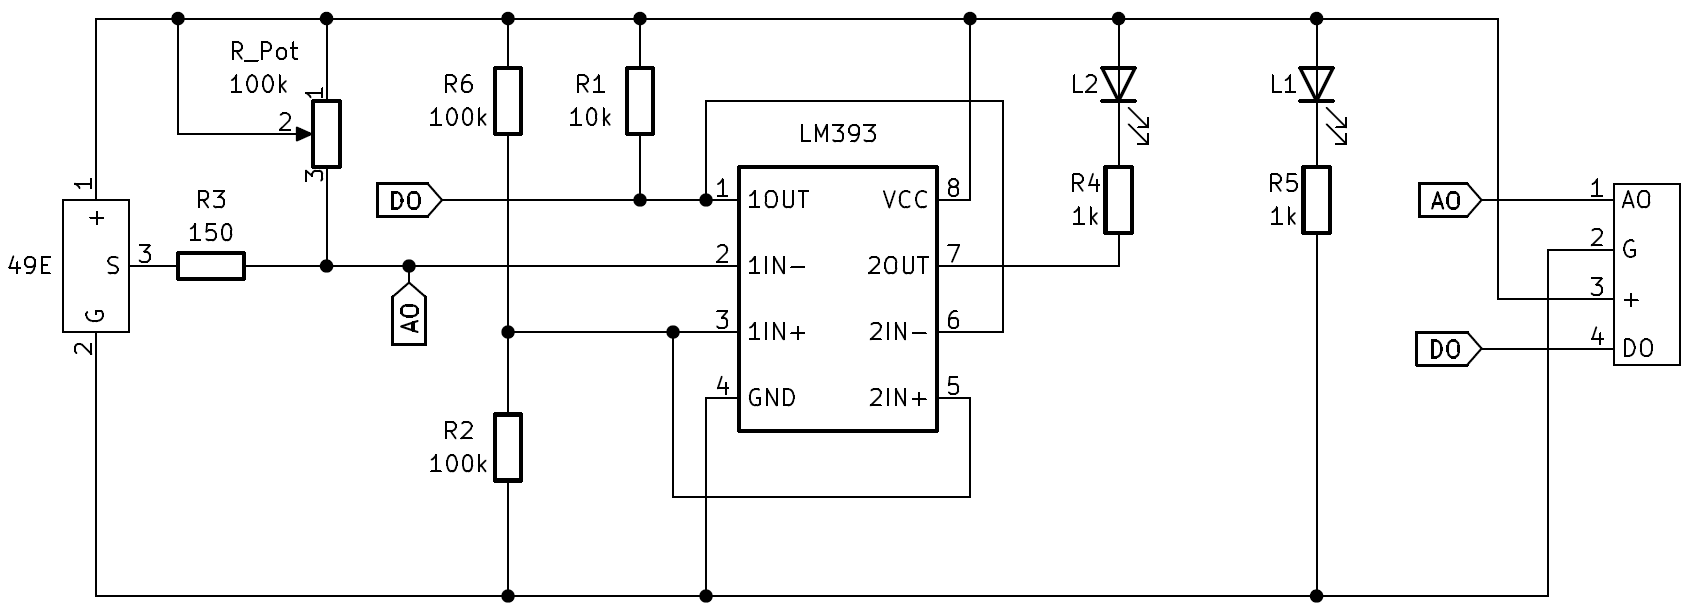
\includegraphics[width=1.0\textwidth]{fig/KY-024/polaczenie_modulu/schematics_internal.png}
    \caption{Schemat budowy wewnętrznej modułu}
    \label{fig:_schemat_modulu}
\end{figure}
\vspace{0.25cm}

Zasada działania czujnika bazuje na kierunkach linii pola magnetycznego (\ref{fig:_zasada_pole_mag}). Włączenie diody LD2 zależne jest od pozycji potencjometru (czułości) i kierunku pola magnetycznego przechodzącego przez detektor. Potencjometr należy wyregulować tak, aby dioda LD1 była zgaszona, gdy czujnik nie znajduje się w polu magnetycznym. Aby włączyć diodę LD2 pole magnetyczne musi przechodzić od dołu (strony z nazwą czujnika) do góry sensora. Można także zastosować odwrócone działanie - dioda LD2 świeci się, gdy sensor znajduje się poza polem magnetycznym. Nalezy jednak pamiętać, że zmieni się wtedy metoda wyłączania diody LD2 - pole magnetyczne musi przechodzić od góry do dołu detektora. Sposób działania można dostosowywać nastawą potencjometru, zgodnie z wymaganiami.

%%%%%%%%%%%%%%%%%%%%%%%%%  TWO IMAGES SIDE BY SIDE  %%%%%%%%%%%%%%%%%%%%%%%%%%%%%
\vspace{0.25cm}
\begin{figure}[h]
\centering
%%%%%%%%%%%%%%%%%%%%%%%%%%%%%%%%%%%%%%%%%%%%%%%%%%%%%%%%%%%%%%%%%%%%%%%%%%%%%%%%%
\begin{subfigure}{.47\textwidth}
\centering
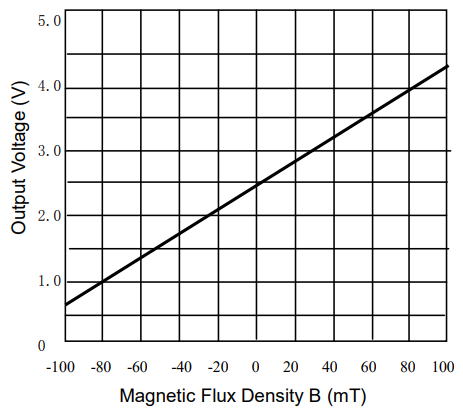
\includegraphics[width=1.0\linewidth]{fig/KY-024/zasada_dzialania/characteristics.png}
\caption{\centering Charakterystyka napięcia wyjściowego czujnika od gęstości strumienia magnetycznego \cite{49E_datasheet}}
\label{fig:_charakterystyka}
\end{subfigure}%
%%%%%%%%%%%%%%%%%%%%%%%%%%%%%%%%%%%%%%%%%%%%%%%%%%%%%%%%%%%%%%%%%%%%%%%%%%%%%%%%%
\begin{subfigure}{.6\textwidth}
\centering
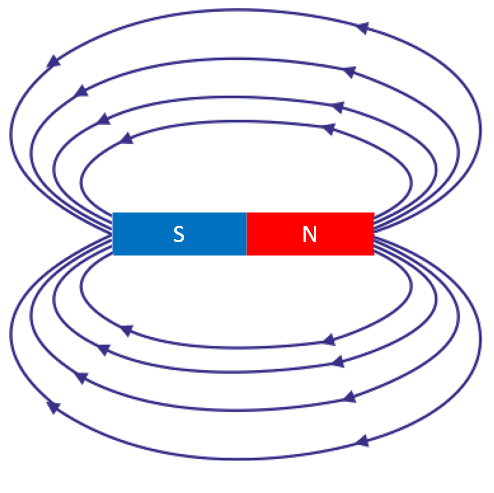
\includegraphics[width=.7\linewidth]{fig/KY-024/zasada_dzialania/pole_mag.png}
\caption{Przebieg linii pola magnetycznego }
\label{fig:_zasada_pole_mag}
\end{subfigure}
%%%%%%%%%%%%%%%%%%%%%%%%%%%%%%%%%%%%%%%%%%%%%%%%%%%%%%%%%%%%%%%%%%%%%%%%%%%%%%%%%
% \caption{PODPIS}
\label{fig:element}
\end{figure}
\vspace{0.25cm}
%%%%%%%%%%%%%%%%%%%%%%%%%  TWO IMAGES SIDE BY SIDE  %%%%%%%%%%%%%%%%%%%%%%%%%%%%%
Działanie układu sygnalizuje dioda L1 - świeci się ona, gdy na wejście '+' podane zostanie odpowiednie napięcie zasilania. Napięcie wyjściowe z czujnika Halla w punkcie 'S' na schemacie (\ref{fig:_schemat_modulu}) jest liniowo zależne od gęstości strumienia indukcji magnetycznej, zgodnie z charakterystyką (\ref{fig:_charakterystyka}). Jeśli pole magnetyczne przebiega od góry do dołu detektora i dioda LD2 jest domyślnie wyłączona, napięcie wyjściowe czujnika Halla zmniejsza się. W związku z tym, potencjał w punkcie AO maleje. Równe wartości rezystorów R6 i R2 powodują podanie połowy napięcia zasilającego na wejścia komparatorów 1IN+ i 2IN+. Gdy napięcie referencyjne z wejścia 1IN- komparatora spadnie poniżej napięcia na wejściu 1IN+, wyjście 1OUT zostanie ustawione w stan wysoki równy napięciu zasilania '+'. Stan ten zostaje przeniesiony na wejście odniesienia 2IN- i porównany z wejściem 2IN+ na którym panuje połowa napięcia zasilania. Gdy $V_{2IN-} > V_{2IN+}$ wyjście 2OUT przyjmuje wartość GND (0V). Tworzy się wtedy różnica potencjałów pomiędzy szyną zasilającą a wyjściem 2OUT, co powoduje zaświecenie diody LD2.


\newpage

\section{Użycie czujnika}
Czujnik posiada 4 wyprowadzenia - dwa zasilające i dwa sygnałowe (analogowe AO i cyfrowe DO). Na rys. \ref{fig:_zdjecie_elementu} przedstawiono oznaczenia wyprowadzeń rzeczywistego czujnika. Działanie czujnika można zweryfikować z użyciem miernika i mikrokontrolera.
\\
Poniżej przedstawiono pomiary wyjścia cyfrowego i analogowego wykonane miernikiem:
\begin{itemize}
\item{Pomiary wyjścia cyfrowego DO - dioda LD2 domyślnie wyłączona, gdy brak pola magnetycznego}
%%%%%%%%%%%%%%%%%%%%%%%%%  TWO IMAGES SIDE BY SIDE  %%%%%%%%%%%%%%%%%%%%%%%%%%%%%
\begin{figure}[h]
\centering
%%%%%%%%%%%%%%%%%%%%%%%%%%%%%%%%%%%%%%%%%%%%%%%%%%%%%%%%%%%%%%%%%%%%%%%%%%%%%%%%%
\begin{subfigure}{.5\textwidth}
\centering
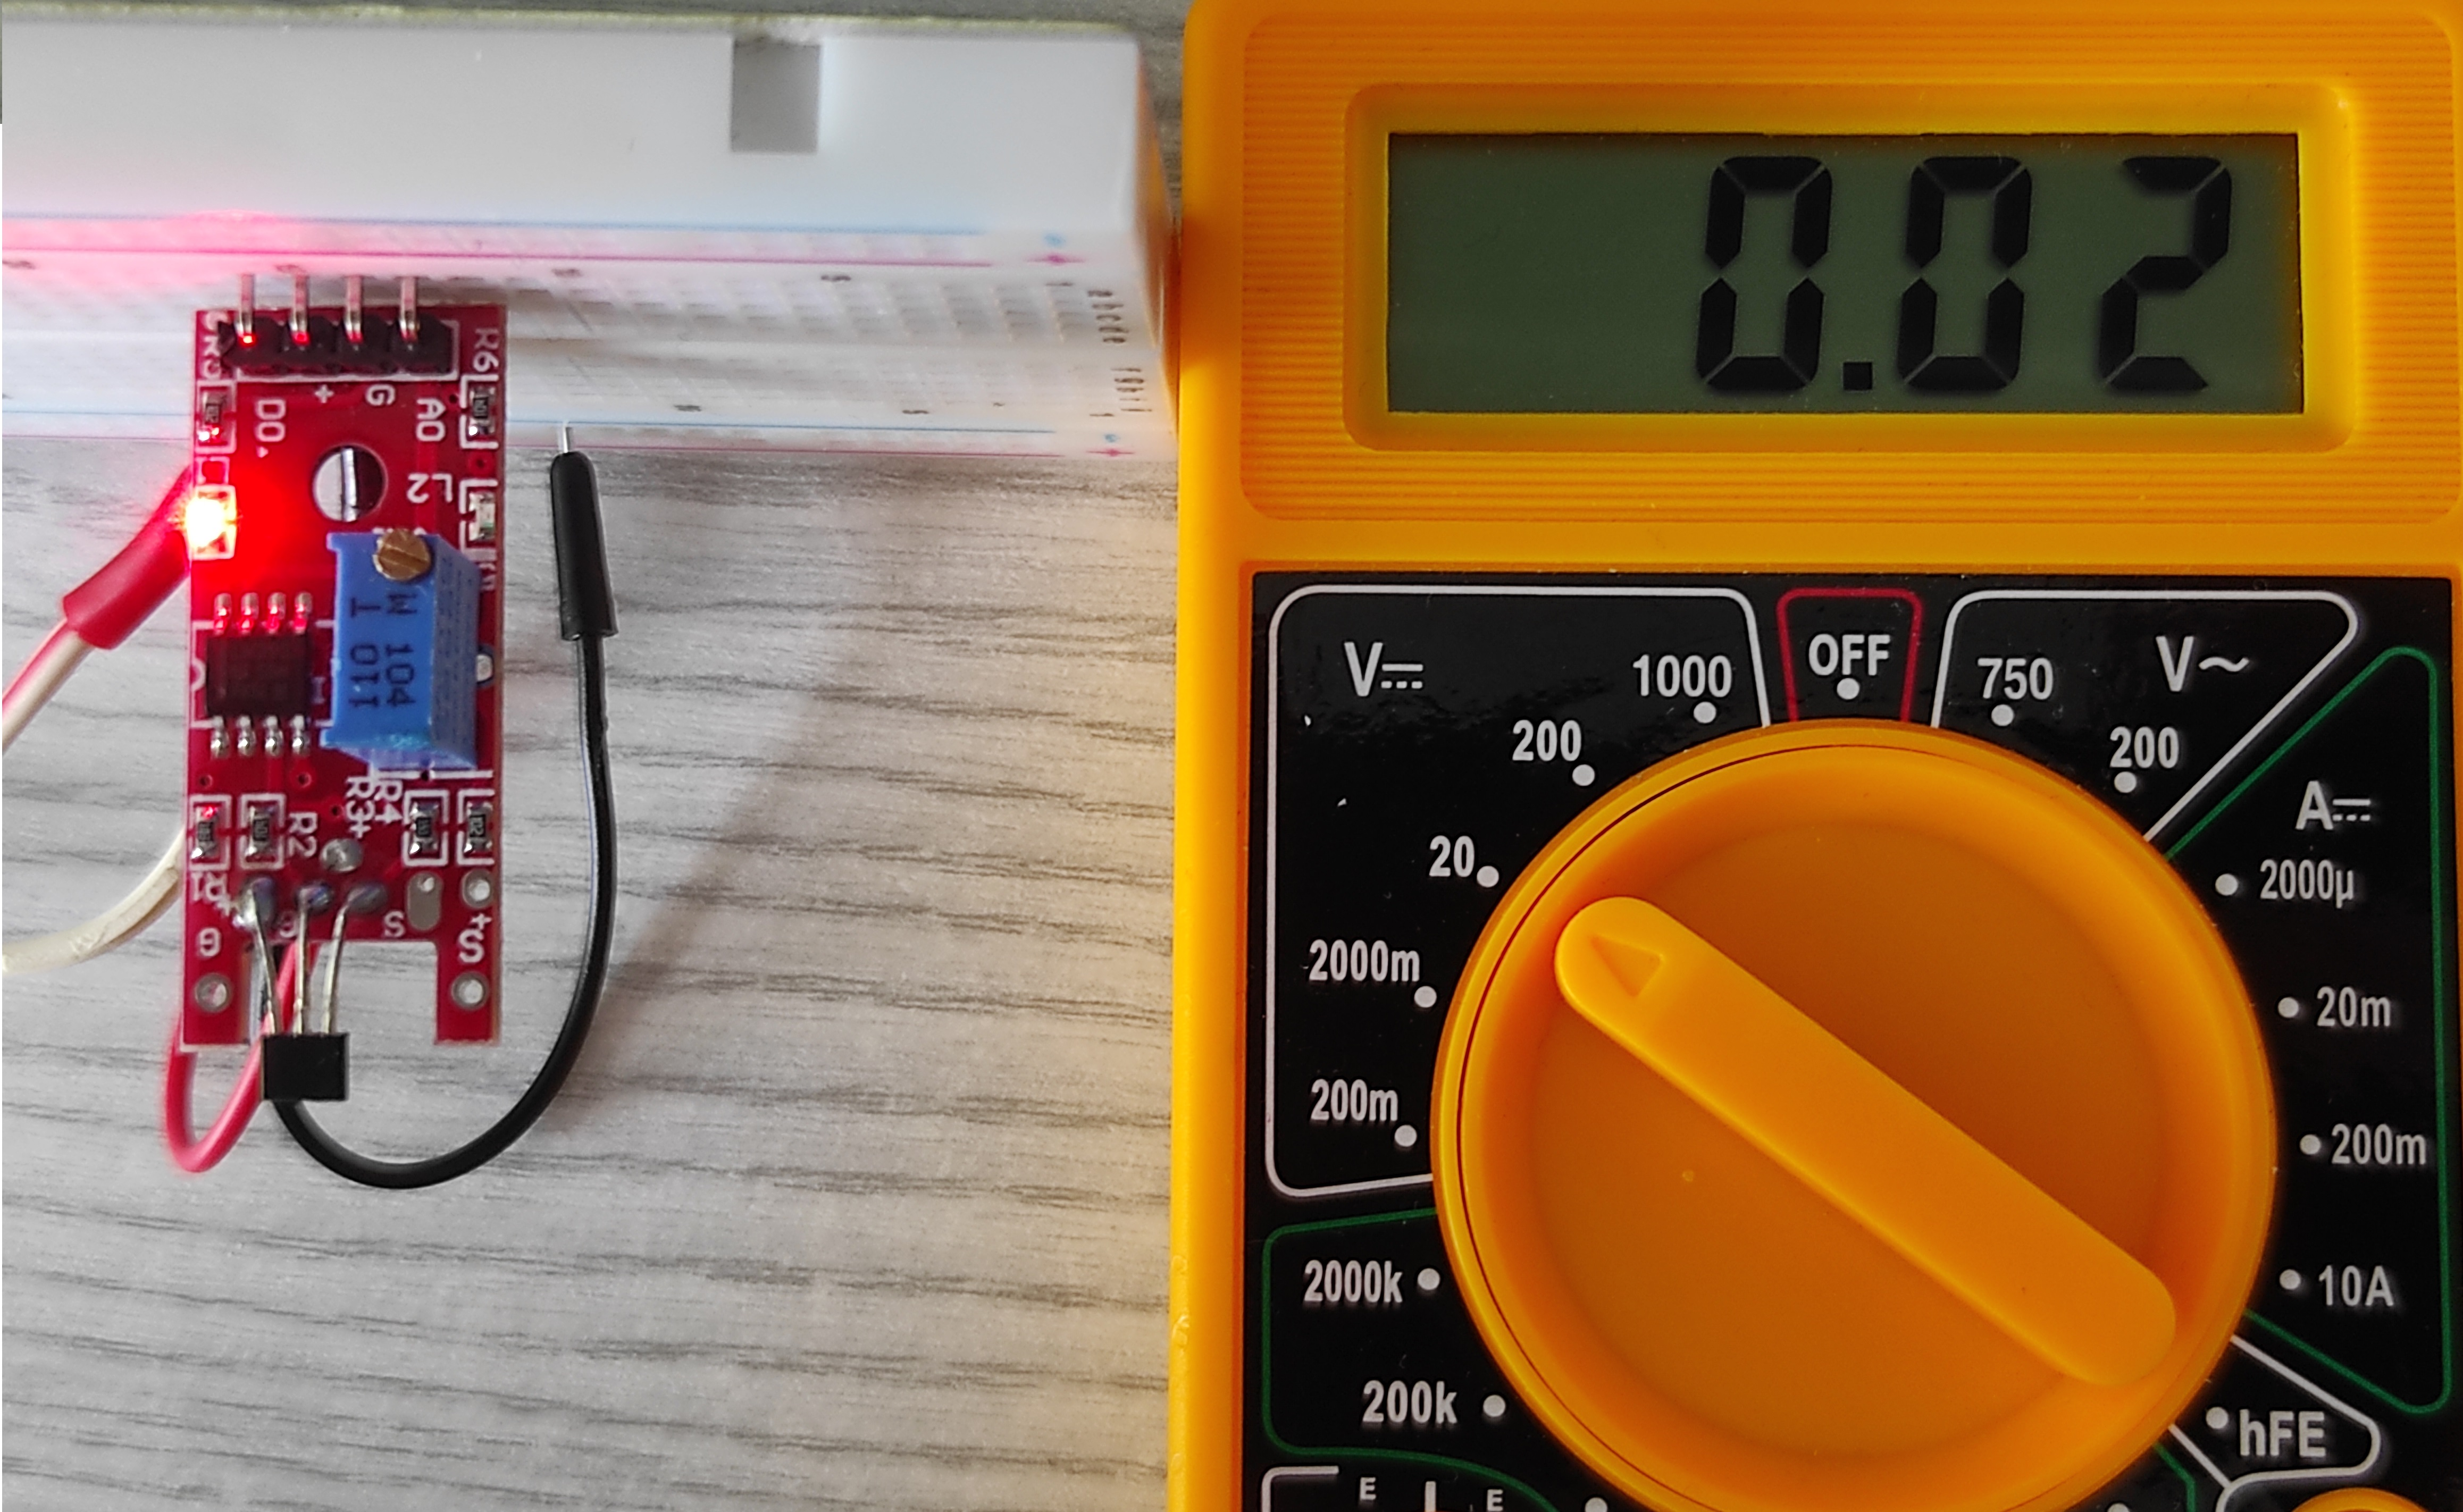
\includegraphics[width=.825\linewidth]{fig/KY-024/działanie_ukladu/digital_min_def_off.jpg}
\caption{Brak pola magnetycznego - stan niski na DO}
\label{fig:_digital_min_def_off}
\end{subfigure}%
%%%%%%%%%%%%%%%%%%%%%%%%%%%%%%%%%%%%%%%%%%%%%%%%%%%%%%%%%%%%%%%%%%%%%%%%%%%%%%%%%
\begin{subfigure}{.5\textwidth}
\centering
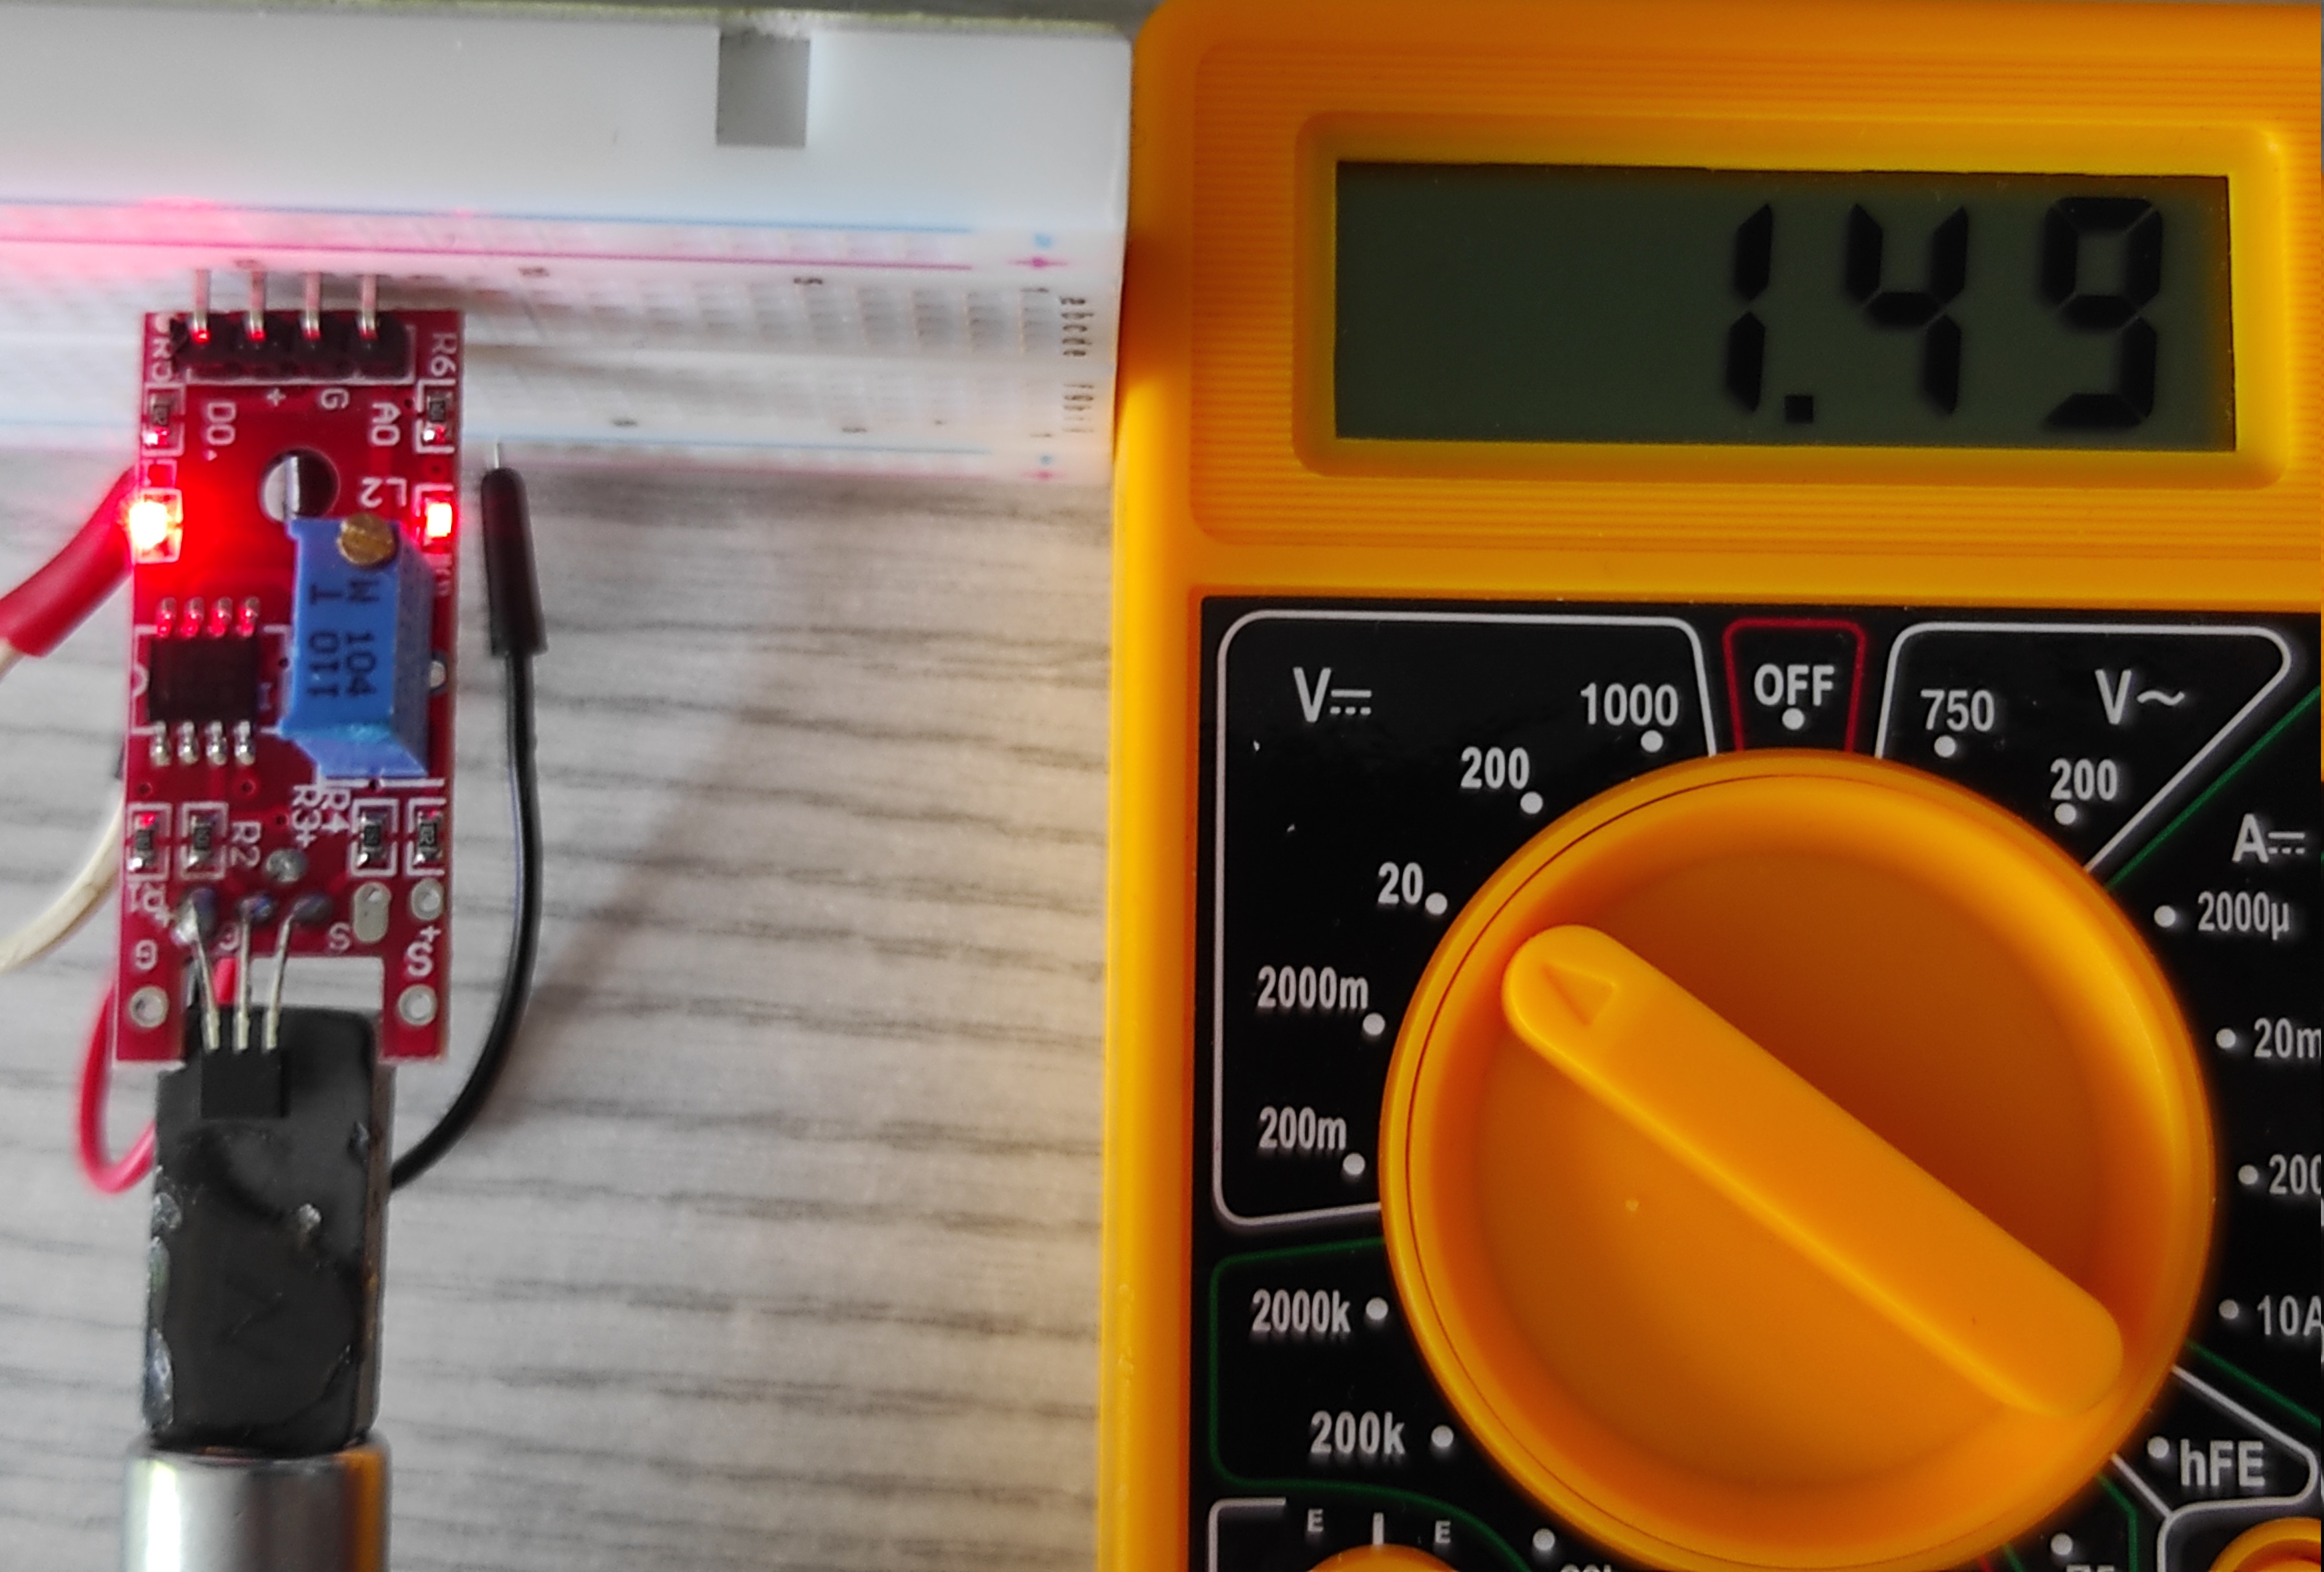
\includegraphics[width=.76\linewidth]{fig/KY-024/działanie_ukladu/digital_max_def_off.jpg}
\caption{Wykrycie pola magnetycznego - stan wysoki na DO}
\label{fig:_digital_max_def_off}
\end{subfigure}
%%%%%%%%%%%%%%%%%%%%%%%%%%%%%%%%%%%%%%%%%%%%%%%%%%%%%%%%%%%%%%%%%%%%%%%%%%%%%%%%%
% \caption{PODPIS}
\label{fig:mikroproc}
\end{figure}
%%%%%%%%%%%%%%%%%%%%%%%%%  TWO IMAGES SIDE BY SIDE  %%%%%%%%%%%%%%%%%%%%%%%%%%%%%

\item{Pomiary wyjścia cyfrowego DO - dioda LD2 domyślnie włączona, gdy brak pola magnetycznego}
%%%%%%%%%%%%%%%%%%%%%%%%%  TWO IMAGES SIDE BY SIDE  %%%%%%%%%%%%%%%%%%%%%%%%%%%%%
\begin{figure}[h]
\centering
%%%%%%%%%%%%%%%%%%%%%%%%%%%%%%%%%%%%%%%%%%%%%%%%%%%%%%%%%%%%%%%%%%%%%%%%%%%%%%%%%
\begin{subfigure}{.5\textwidth}
\centering
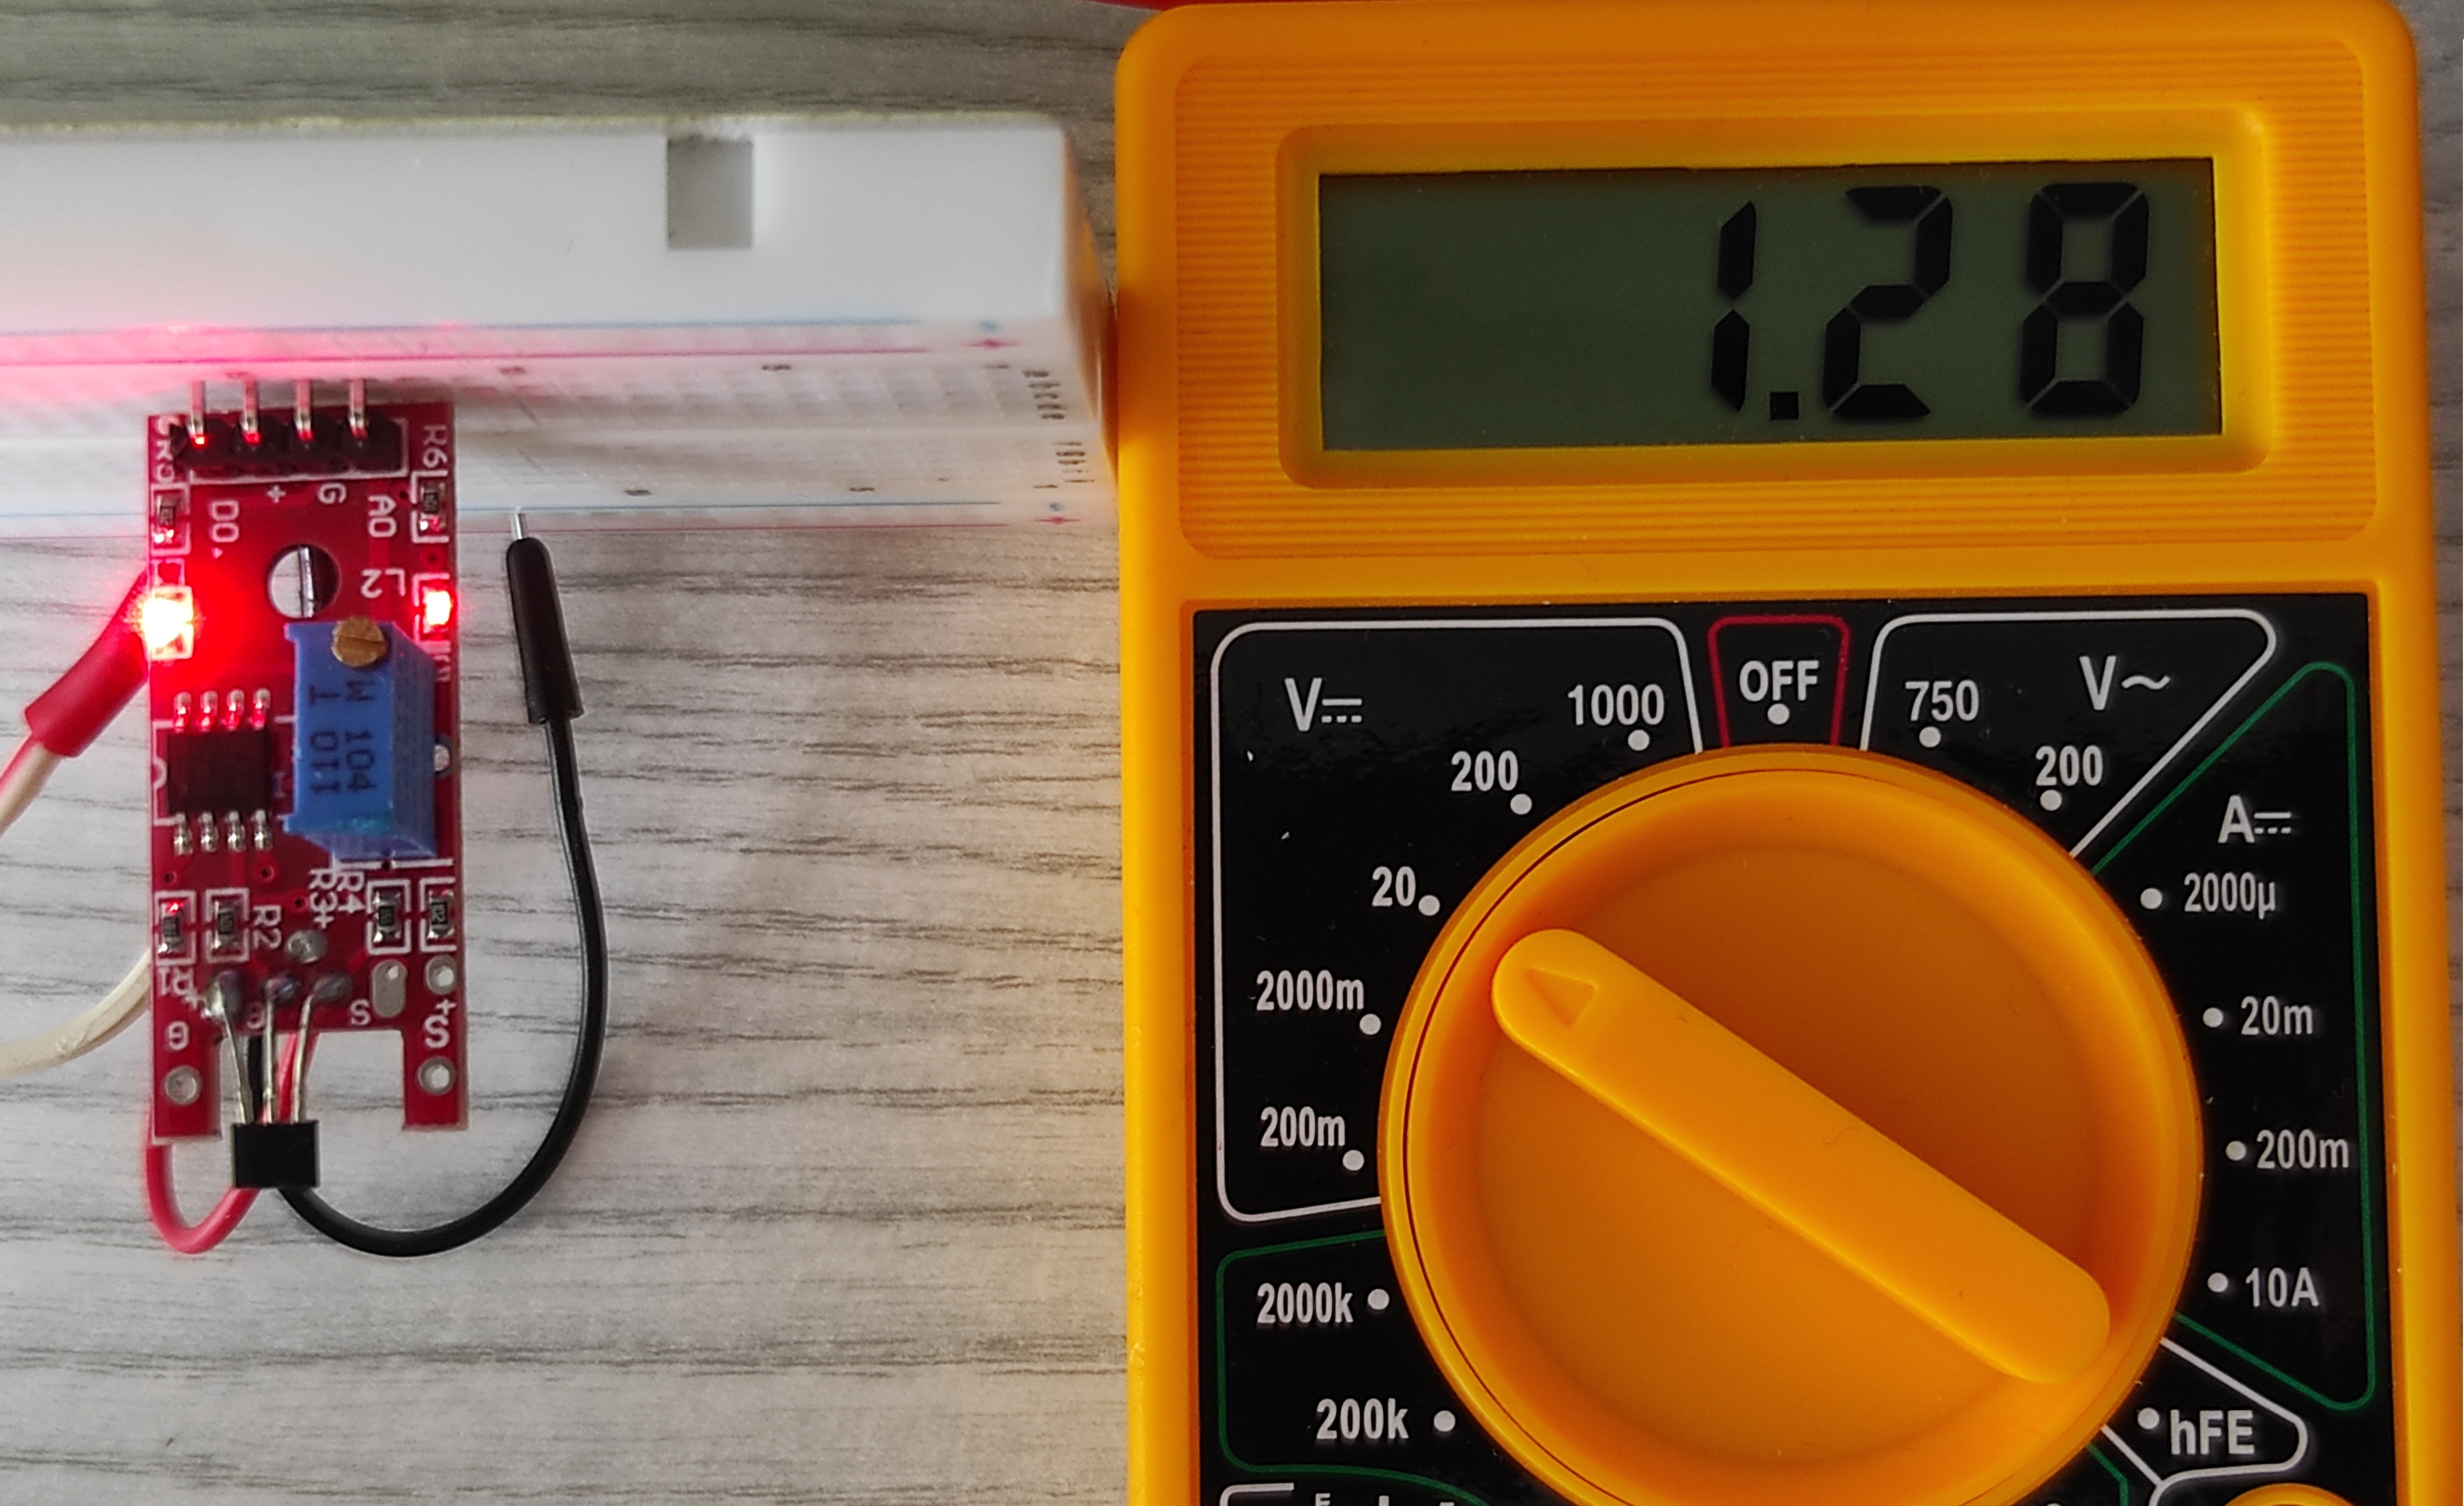
\includegraphics[width=.825\linewidth]{fig/KY-024/działanie_ukladu/digital_mid_def_on.jpg}
\caption{Brak pola magnetycznego - stan wysoki na DO}
\label{fig:_digital_mid_def_on}
\end{subfigure}%
%%%%%%%%%%%%%%%%%%%%%%%%%%%%%%%%%%%%%%%%%%%%%%%%%%%%%%%%%%%%%%%%%%%%%%%%%%%%%%%%%
\begin{subfigure}{.5\textwidth}
\centering
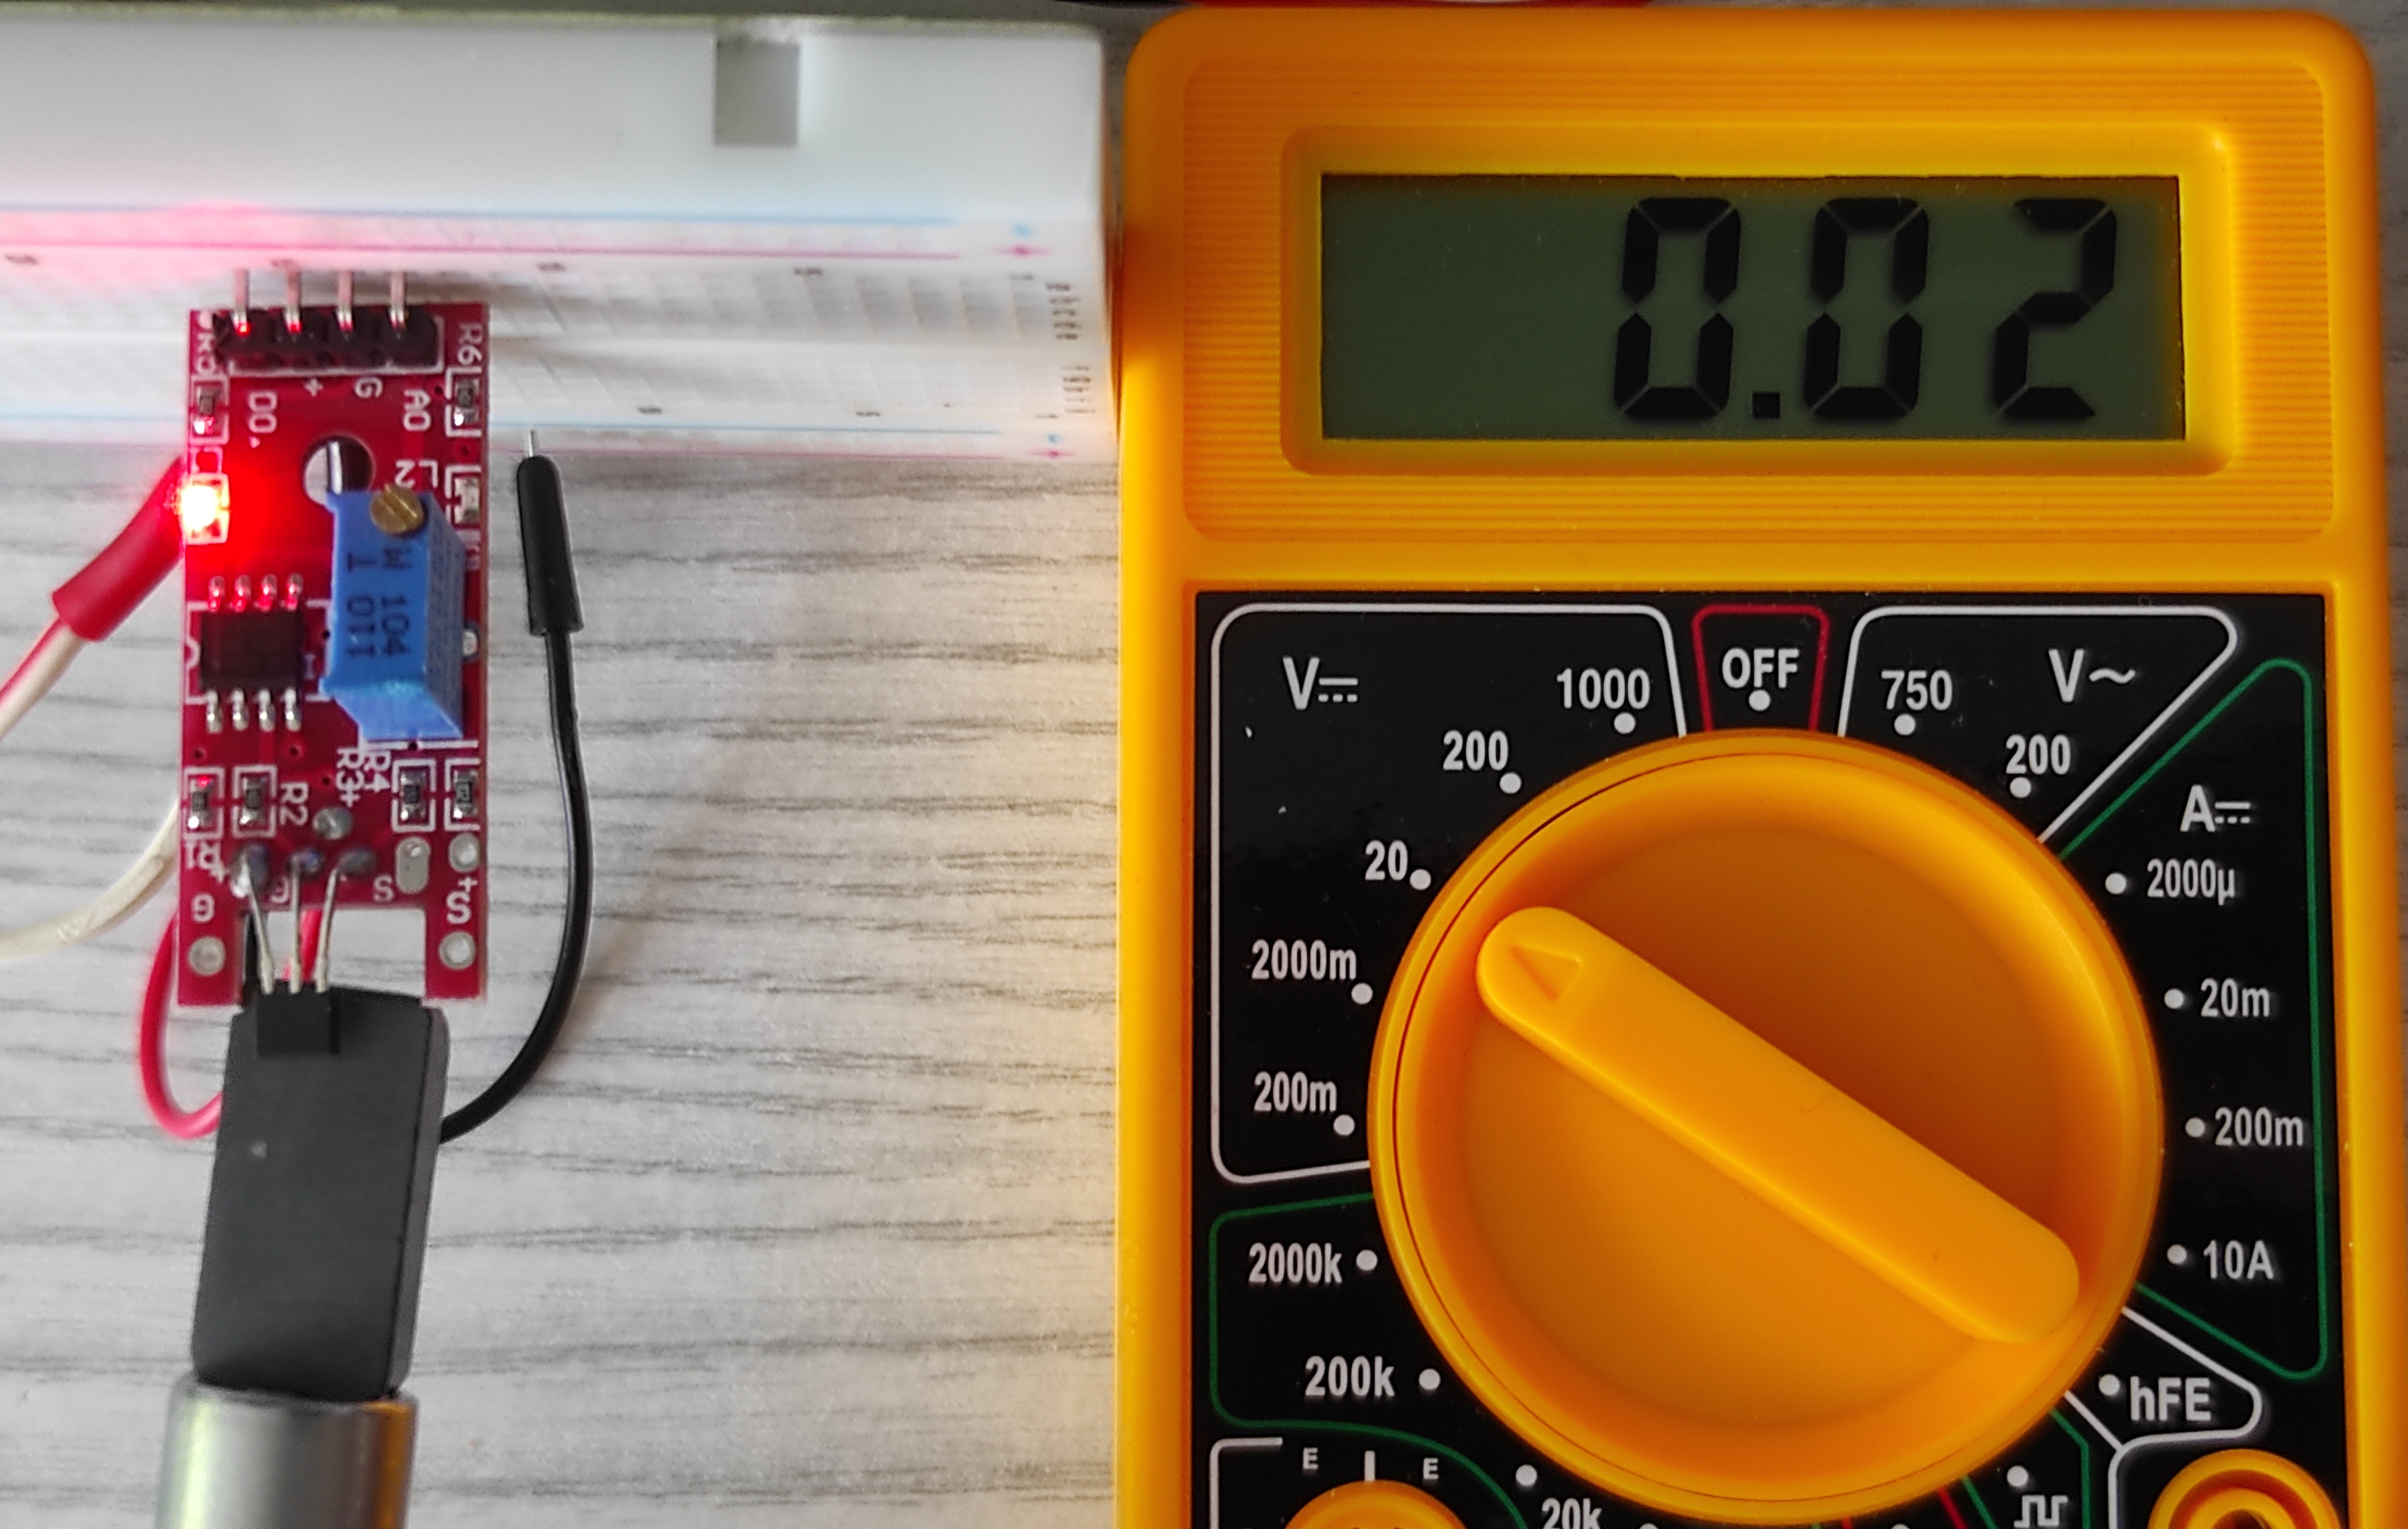
\includegraphics[width=.79\linewidth]{fig/KY-024/działanie_ukladu/digital_min_def_on.jpg}
\caption{Wykrycie pola magnetycznego - stan niski na DO}
\label{fig:_digital_min_def_on}
\end{subfigure}
%%%%%%%%%%%%%%%%%%%%%%%%%%%%%%%%%%%%%%%%%%%%%%%%%%%%%%%%%%%%%%%%%%%%%%%%%%%%%%%%%
% \caption{PODPIS}
\label{fig:miernik2}
\end{figure}
%%%%%%%%%%%%%%%%%%%%%%%%%  TWO IMAGES SIDE BY SIDE  %%%%%%%%%%%%%%%%%%%%%%%%%%%%%

{\color{red}UWAGA: Przyłożenie niewłaściwego bieguna magnesu w trybie domyślnego stanu wysokiego skutkuje wygenerowaniem napięcia bliskiego napięciu zasilania na wyjściu DO, co może prowadzić do przeciążenia GPIO, gdy nie jest odporne na takie napięcia.}

\vspace{0.25cm}
\begin{figure}[h]
    \centering
    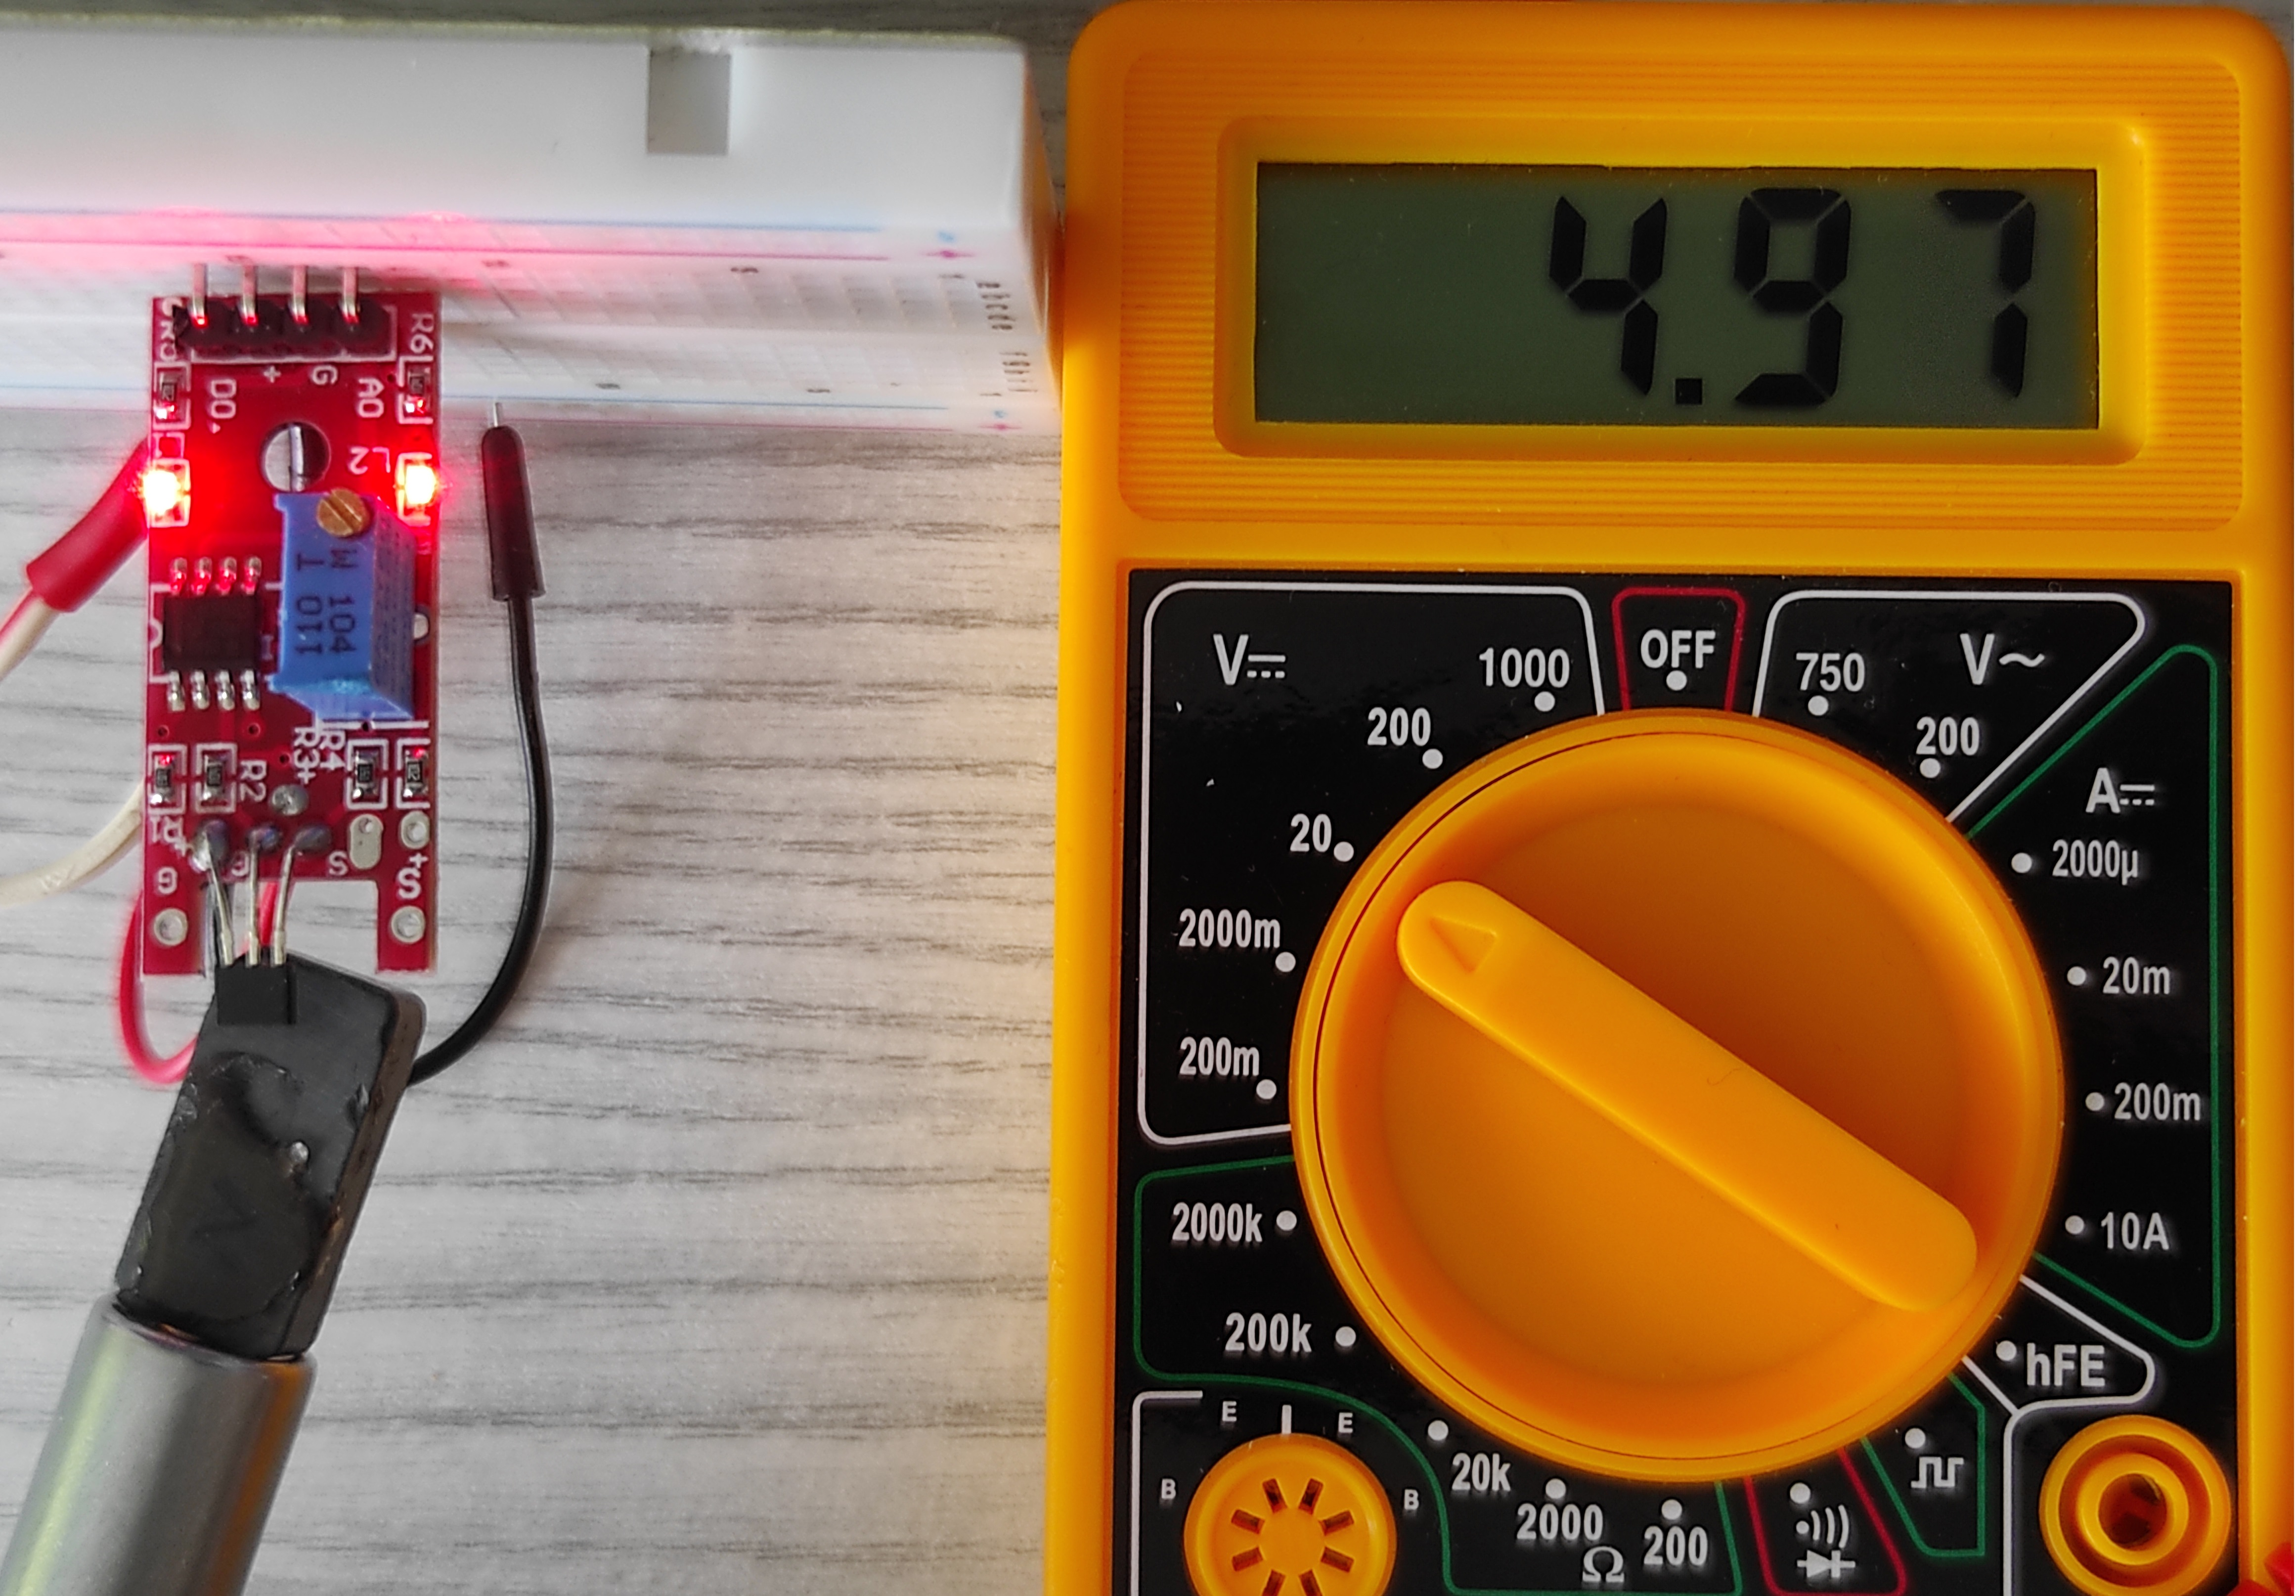
\includegraphics[width=.4\textwidth]{fig/KY-024/działanie_ukladu/digital_max_def_on.jpg}
    \caption{Napięcie zasilania na DO}
    \label{fig:_digital_max_def_on}
\end{figure}
\vspace{0.25cm}

\newpage

\item{Pomiary wyjścia analogowego AO - dioda LD2 domyślnie wyłączona}
%%%%%%%%%%%%%%%%%%%%%%%%%  TWO IMAGES SIDE BY SIDE  %%%%%%%%%%%%%%%%%%%%%%%%%%%%%
\begin{figure}[h]
\centering
%%%%%%%%%%%%%%%%%%%%%%%%%%%%%%%%%%%%%%%%%%%%%%%%%%%%%%%%%%%%%%%%%%%%%%%%%%%%%%%%%
\begin{subfigure}{.5\textwidth}
\centering
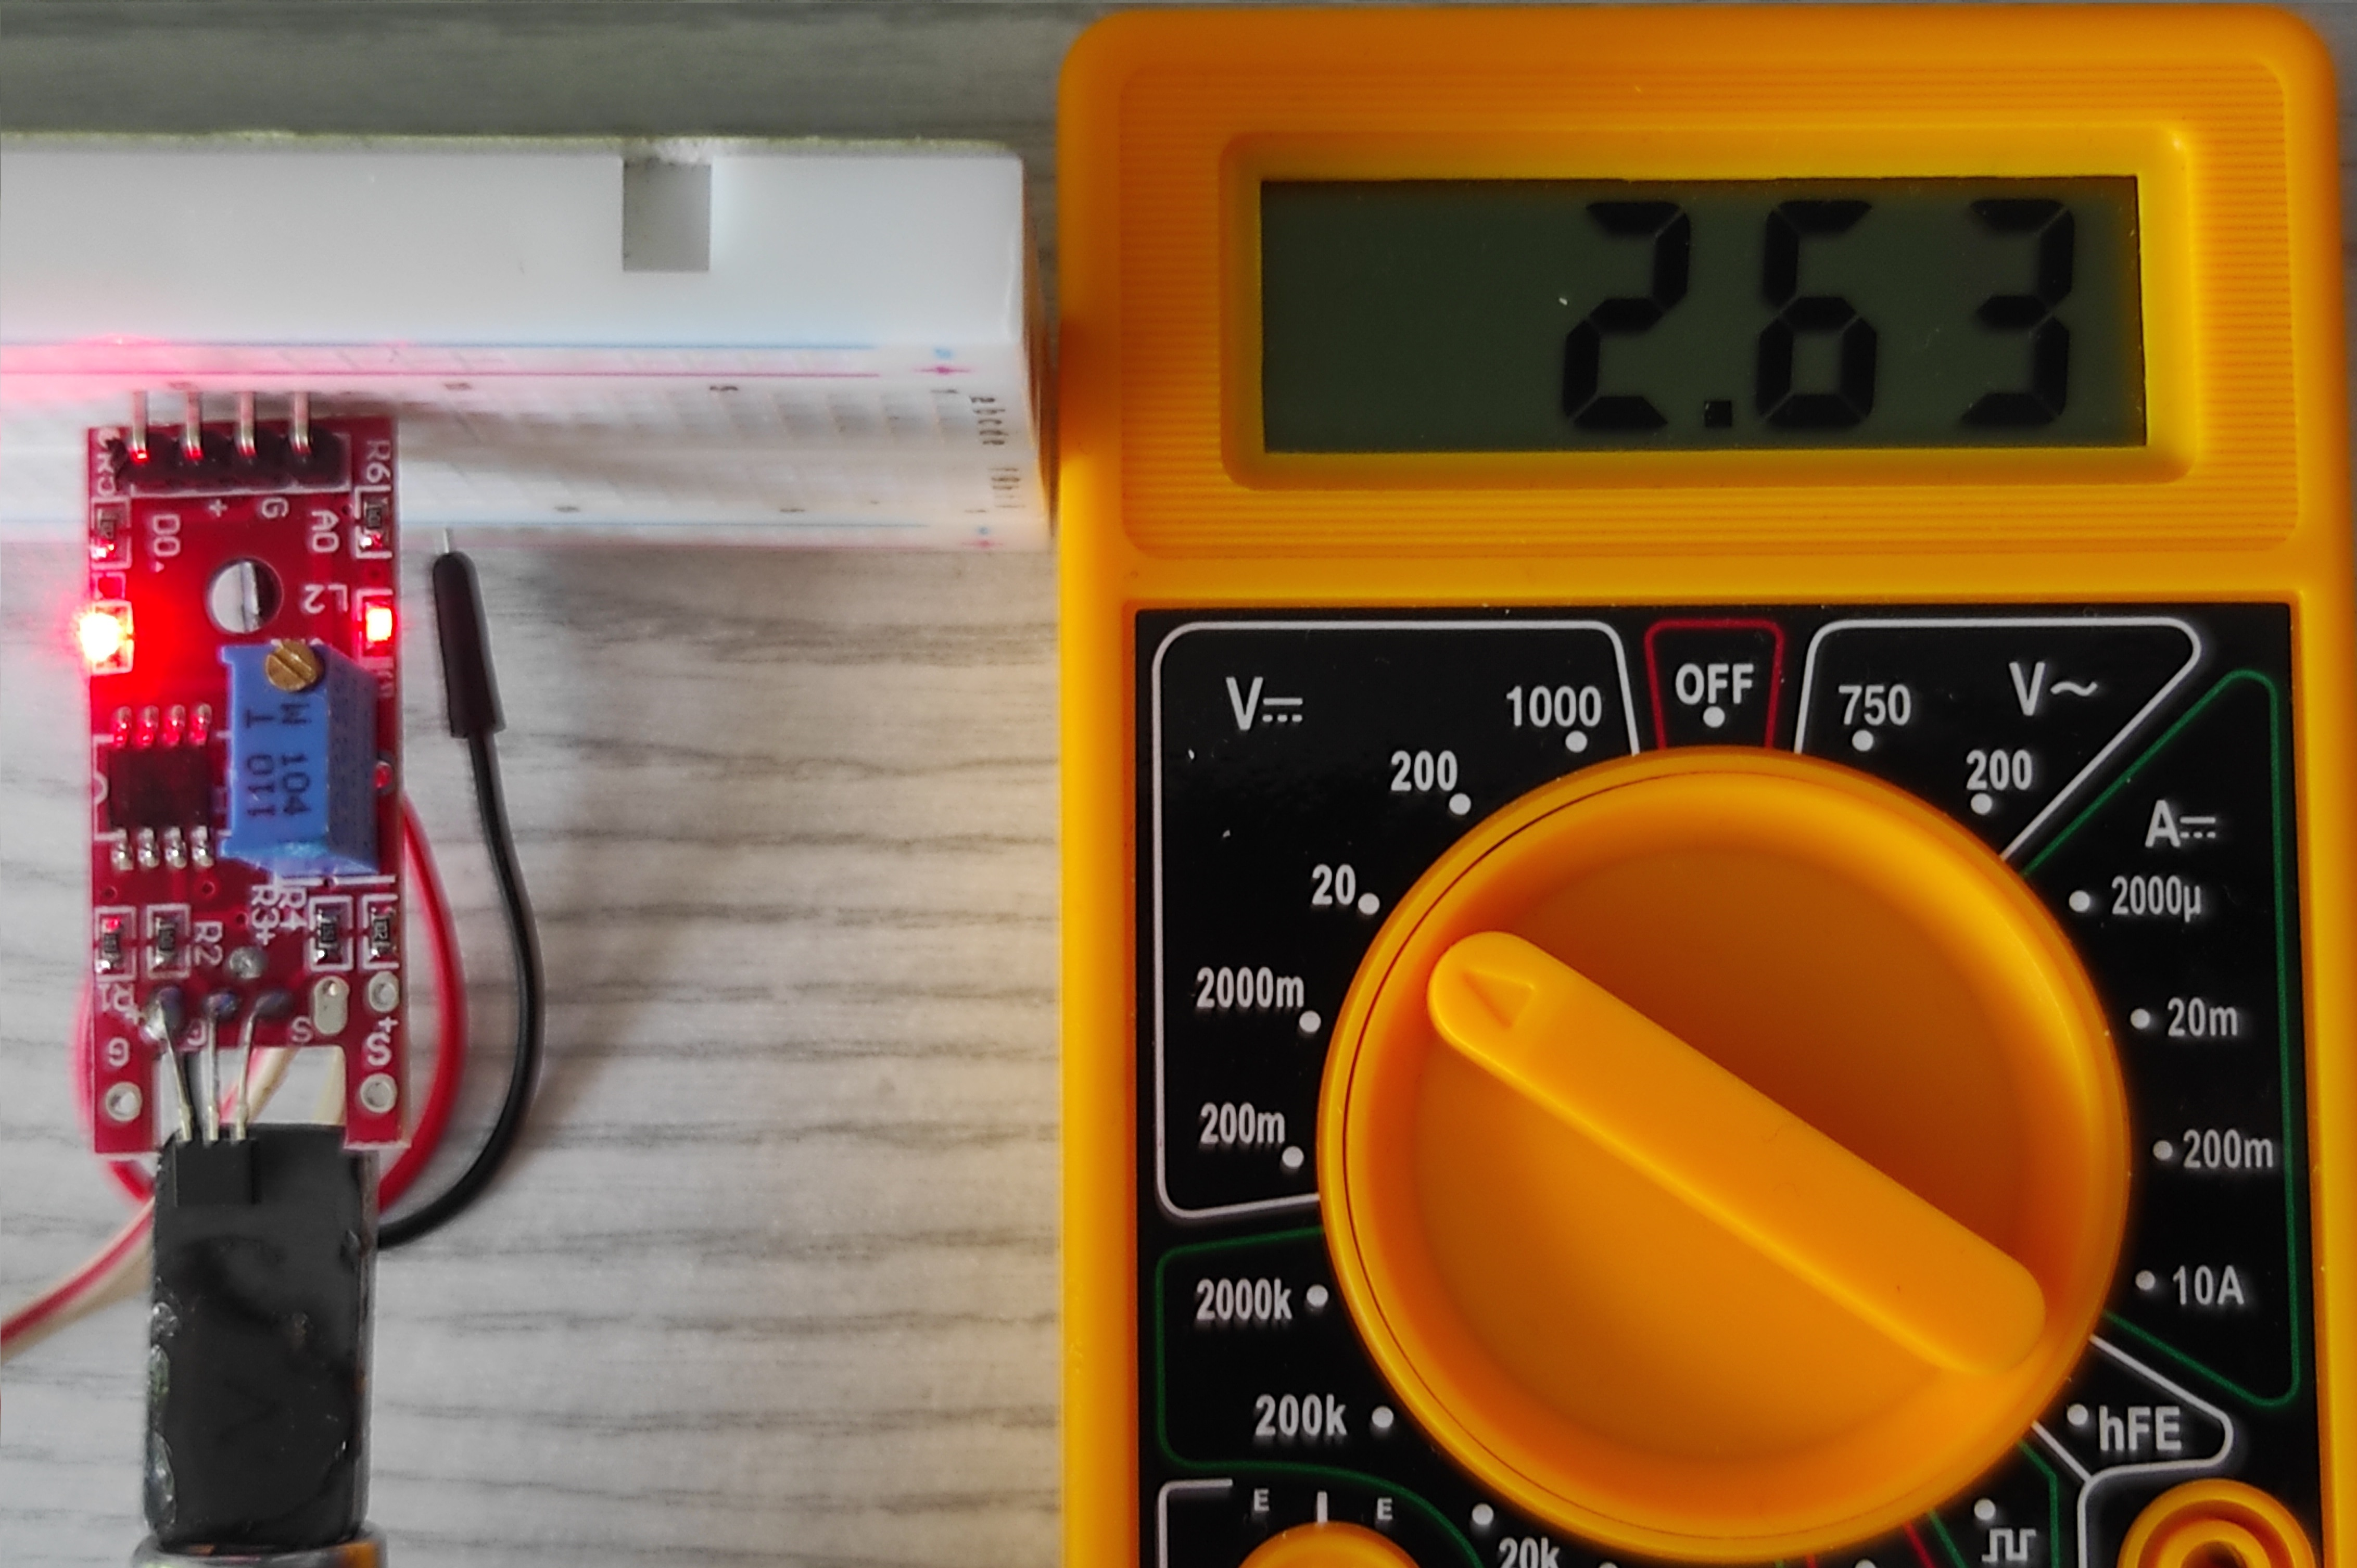
\includegraphics[width=.8\linewidth]{fig/KY-024/działanie_ukladu/analog_min_def_off.jpg}
\caption{Wykrycie bieguna N magnesu}
\label{fig:_analog_min_def_on}
\end{subfigure}%
%%%%%%%%%%%%%%%%%%%%%%%%%%%%%%%%%%%%%%%%%%%%%%%%%%%%%%%%%%%%%%%%%%%%%%%%%%%%%%%%%
\begin{subfigure}{.5\textwidth}
\centering
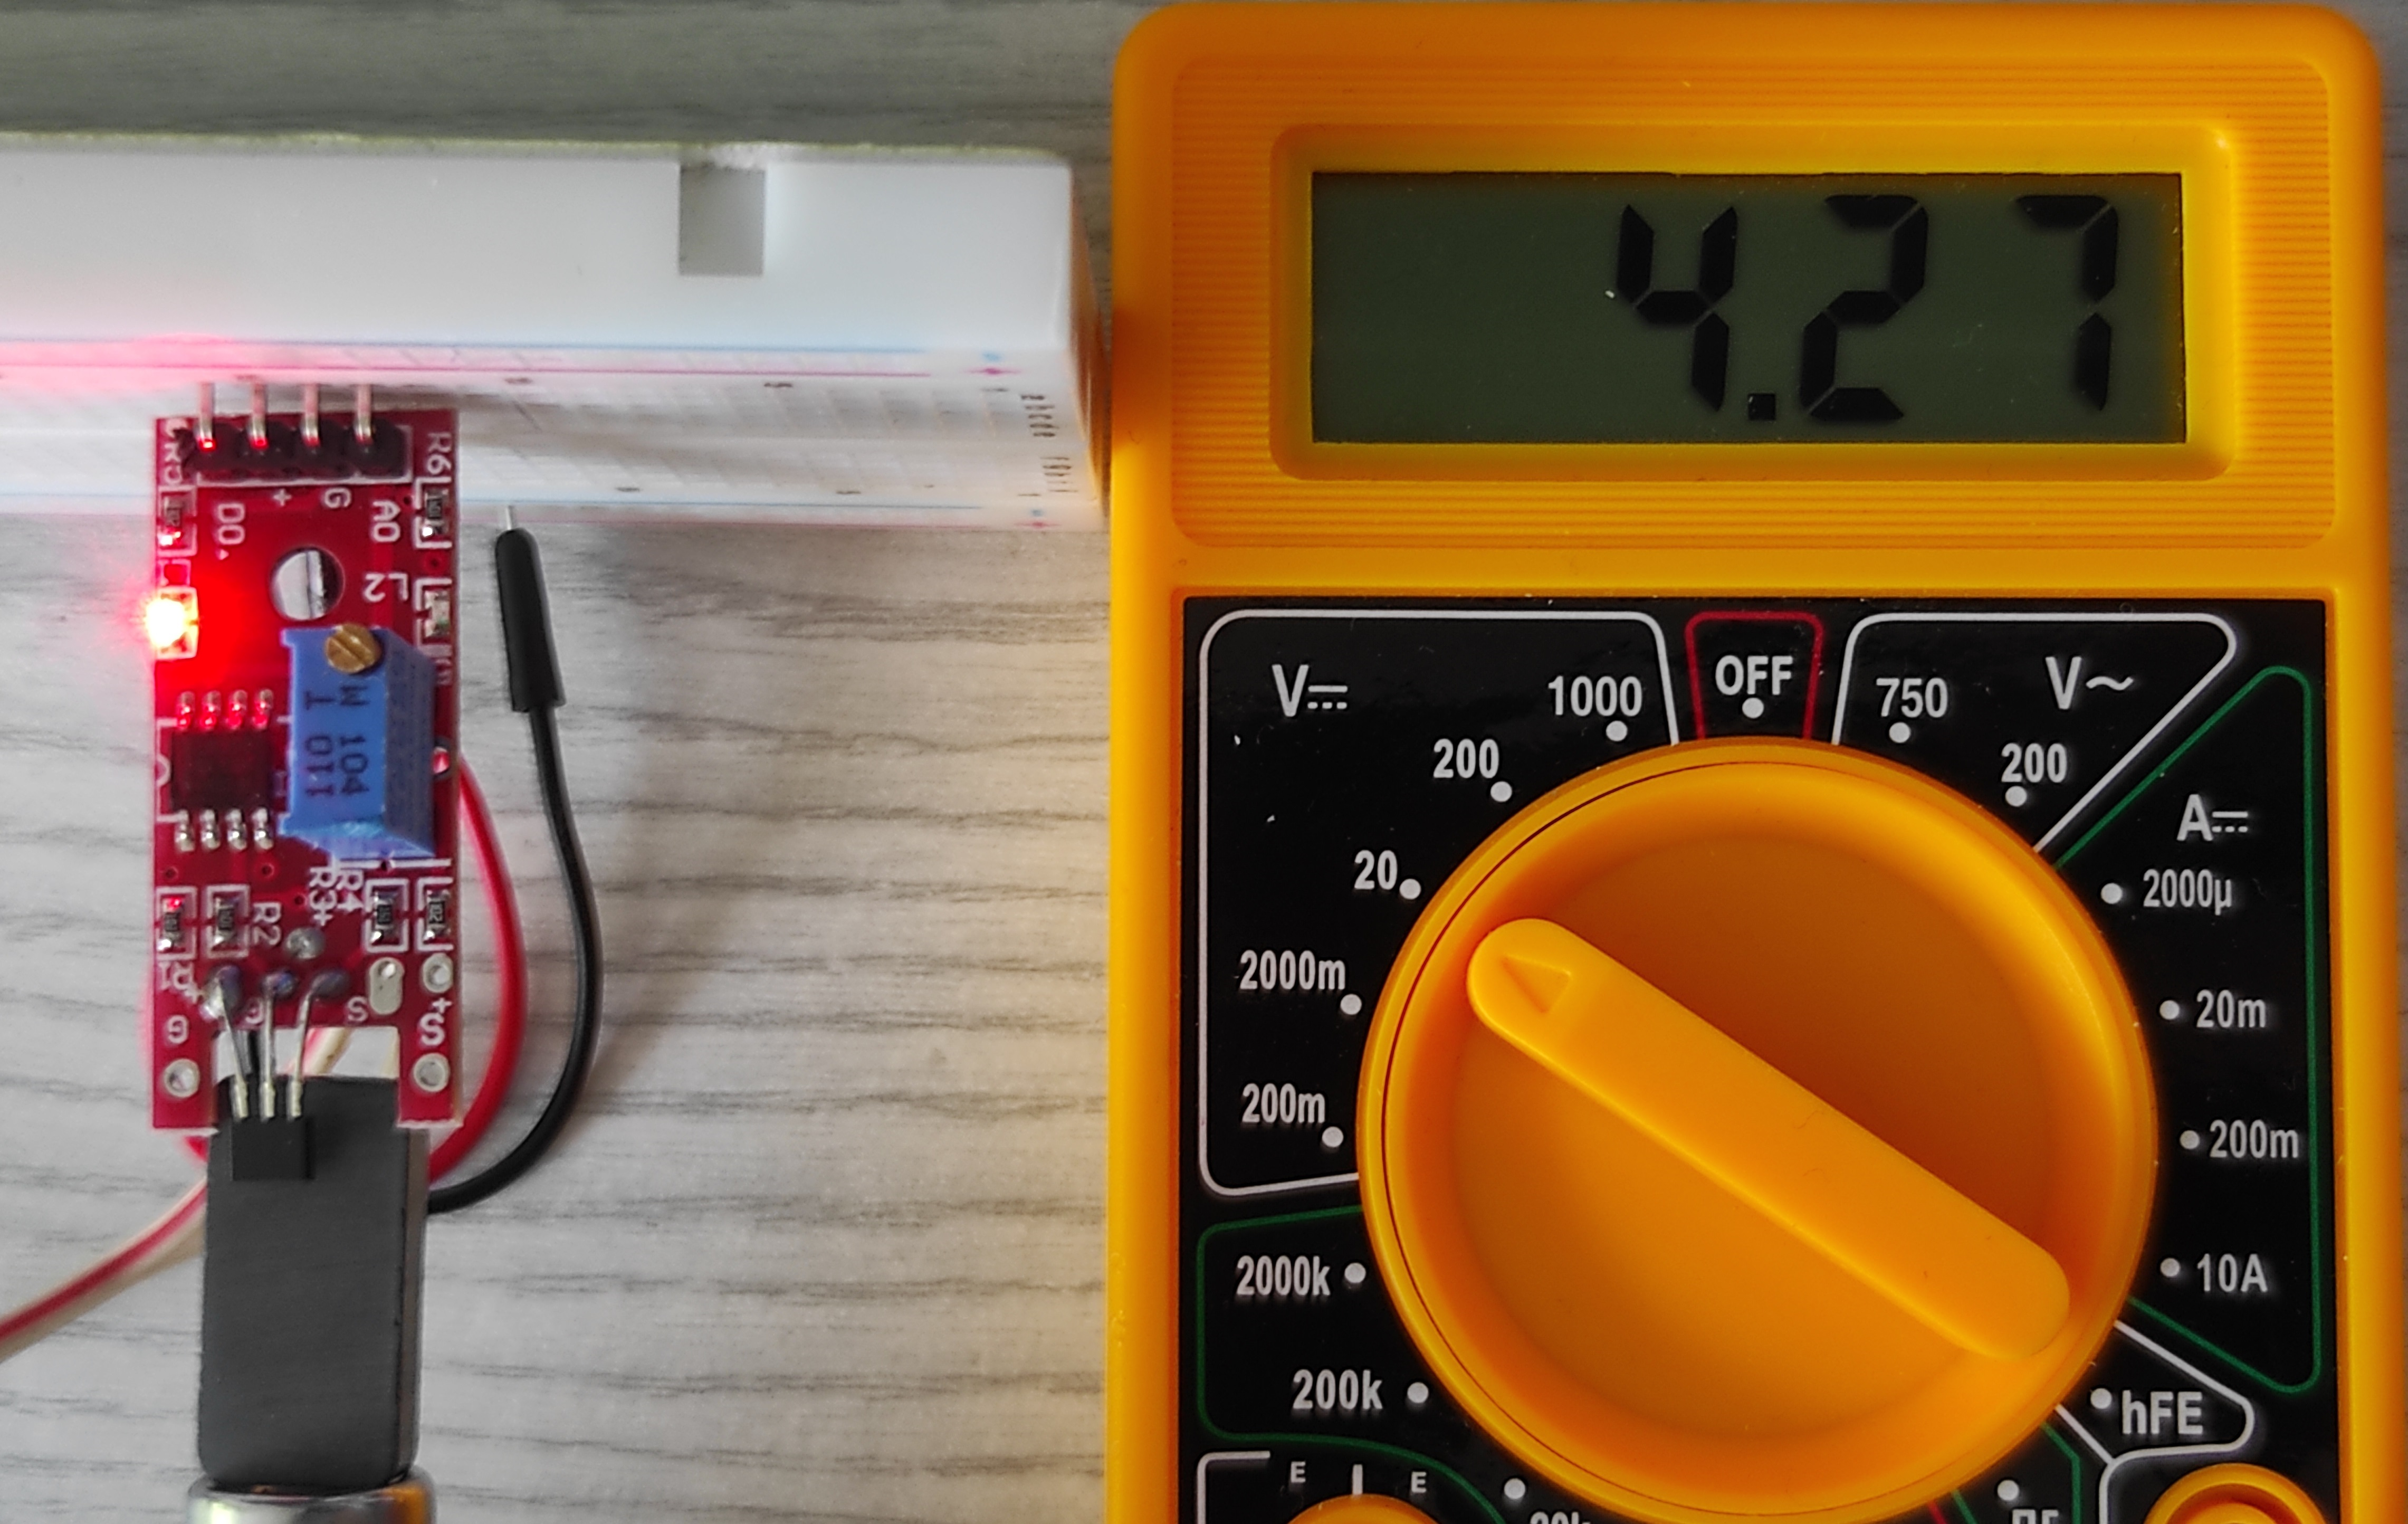
\includegraphics[width=.83\linewidth]{fig/KY-024/działanie_ukladu/analog_max_def_off.jpg}
\caption{Wykrycie bieguna S magnesu}
\label{fig:_analog_max_def_on}
\end{subfigure}
%%%%%%%%%%%%%%%%%%%%%%%%%%%%%%%%%%%%%%%%%%%%%%%%%%%%%%%%%%%%%%%%%%%%%%%%%%%%%%%%%
% \caption{PODPIS}
\label{fig:miernik3}
\end{figure}
%%%%%%%%%%%%%%%%%%%%%%%%%  TWO IMAGES SIDE BY SIDE  %%%%%%%%%%%%%%%%%%%%%%%%%%%%%

\begin{figure}[h]
    \centering
    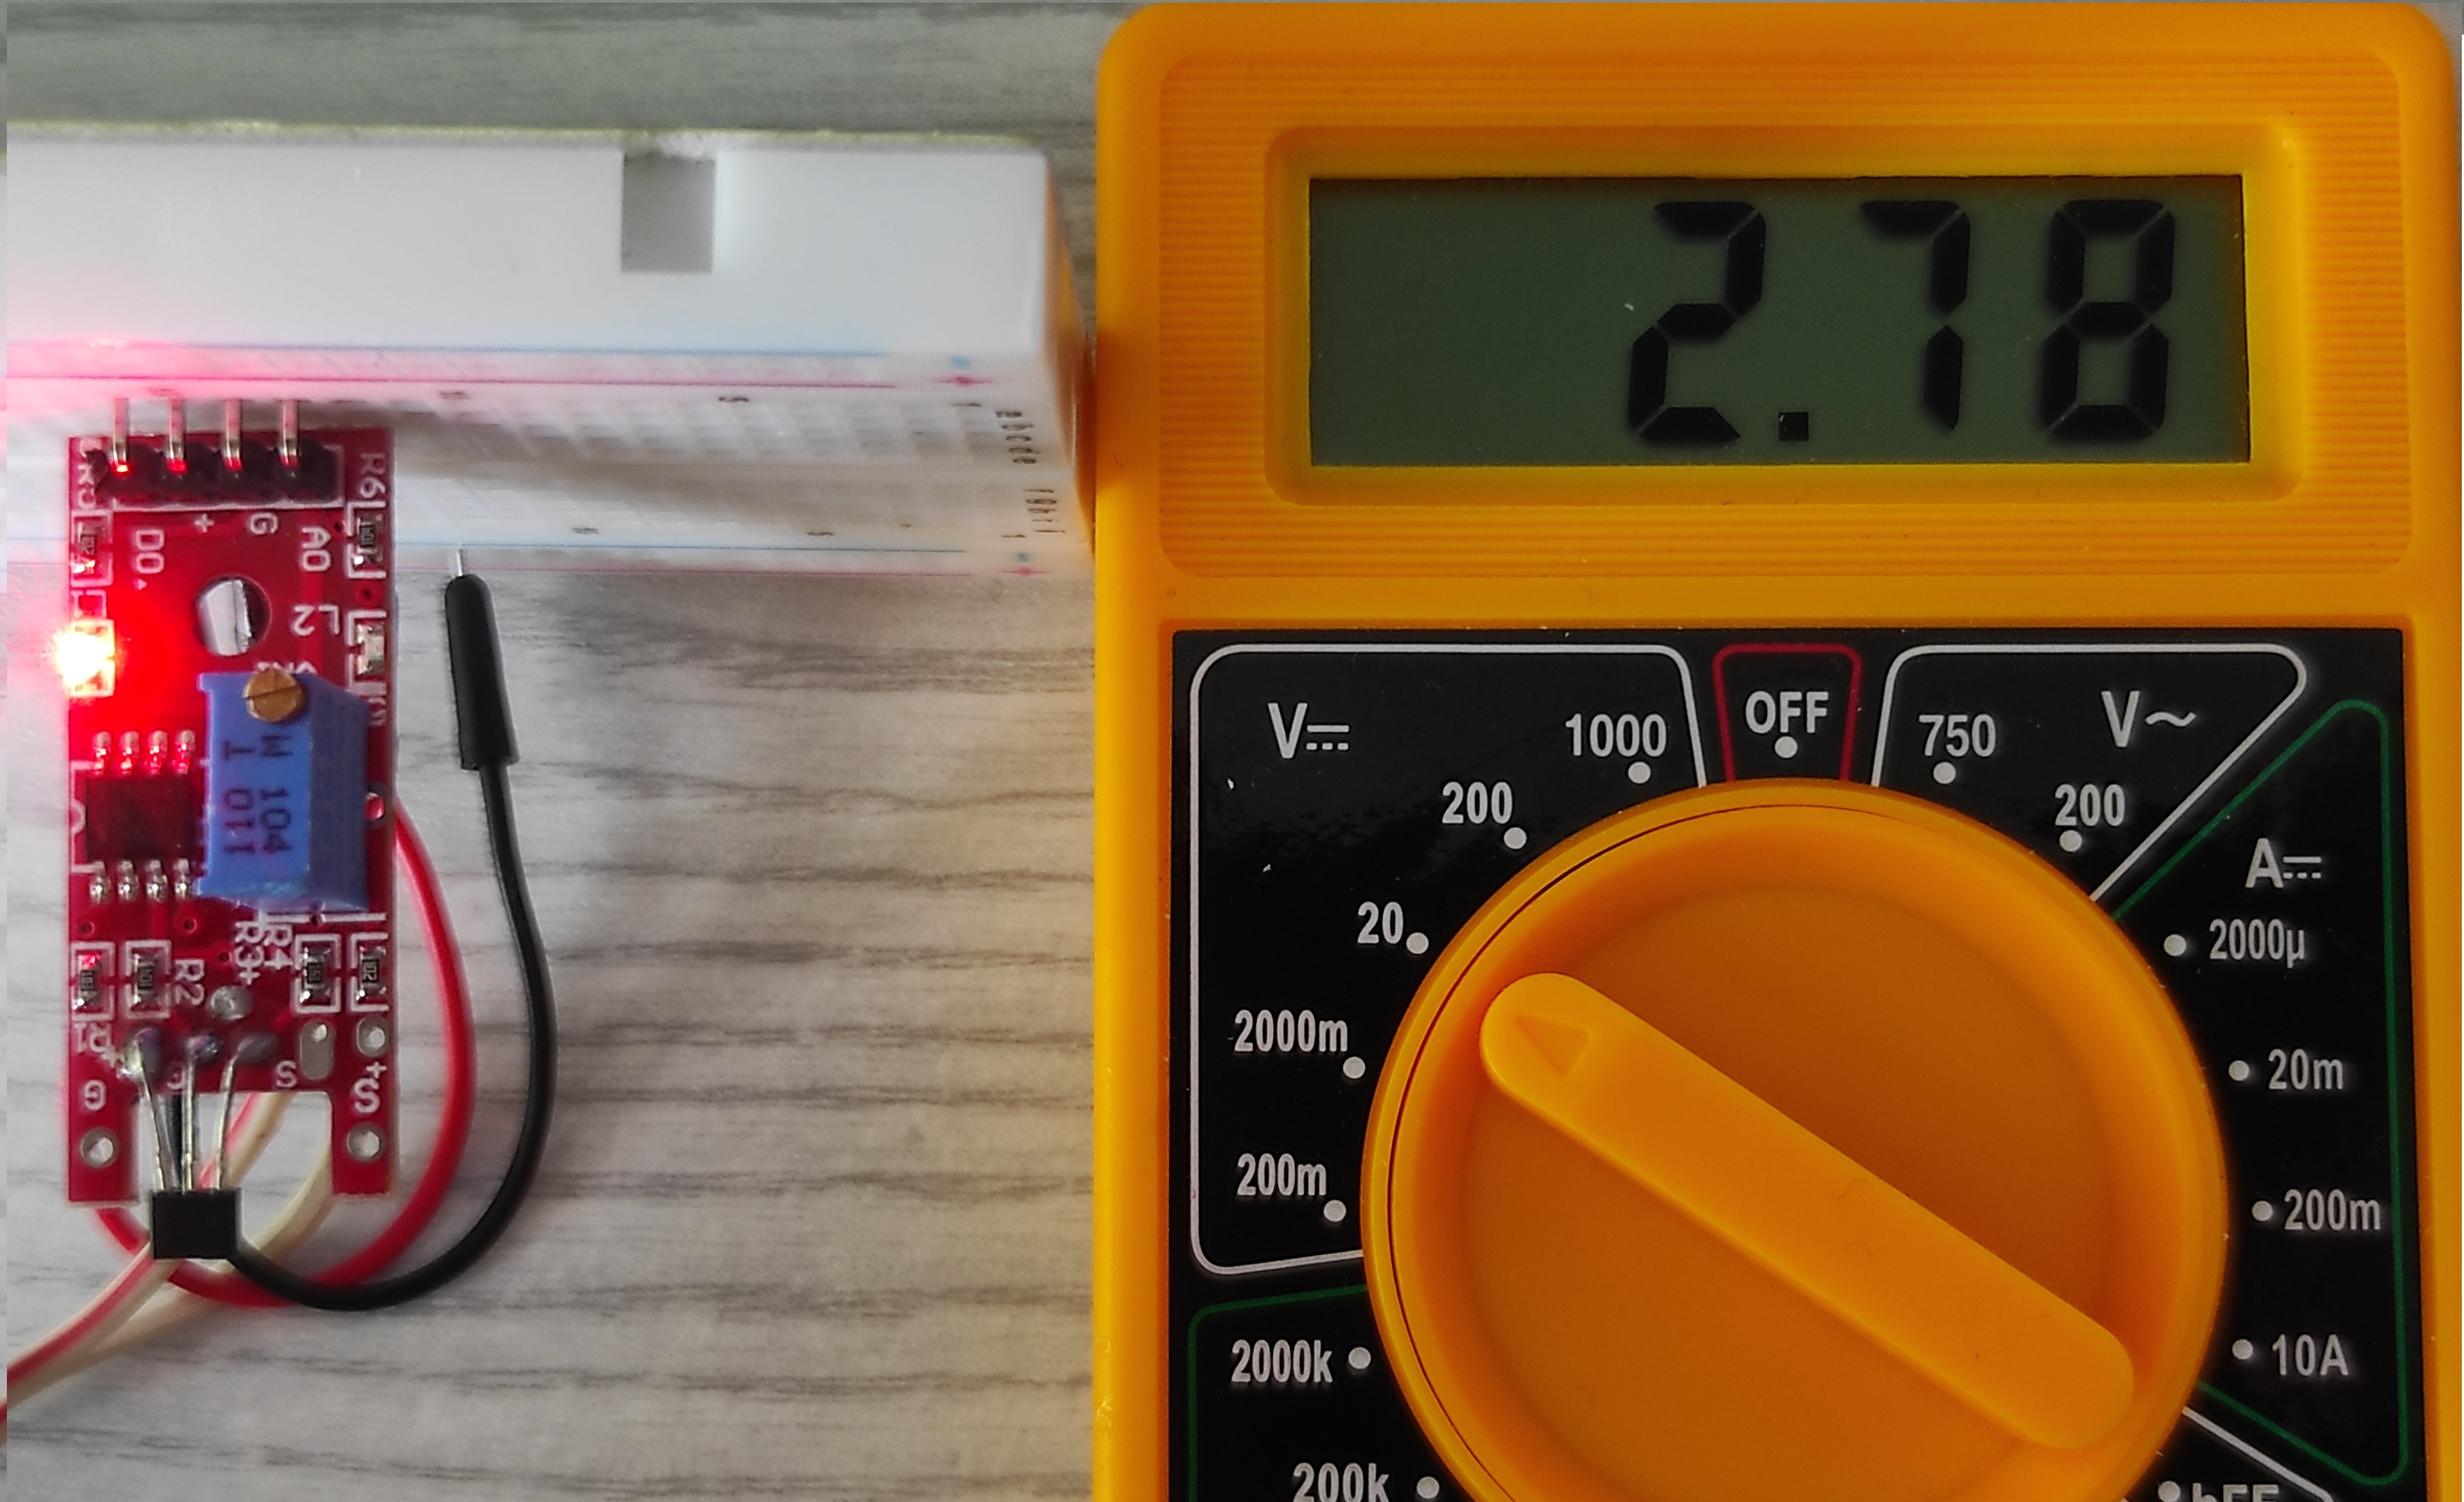
\includegraphics[width=.4\textwidth]{fig/KY-024/działanie_ukladu/analog_mid_def_off.jpg}
    \caption{Brak pola magnetycznego}
    \label{fig:_analog_mid_def_on}
\end{figure}
\vspace{0.25cm}


\item{Pomiary wyjścia analogowego AO - dioda LD2 domyślnie włączona}
%%%%%%%%%%%%%%%%%%%%%%%%%  TWO IMAGES SIDE BY SIDE  %%%%%%%%%%%%%%%%%%%%%%%%%%%%%
\begin{figure}[h]
\centering
%%%%%%%%%%%%%%%%%%%%%%%%%%%%%%%%%%%%%%%%%%%%%%%%%%%%%%%%%%%%%%%%%%%%%%%%%%%%%%%%%
\begin{subfigure}{.5\textwidth}
\centering
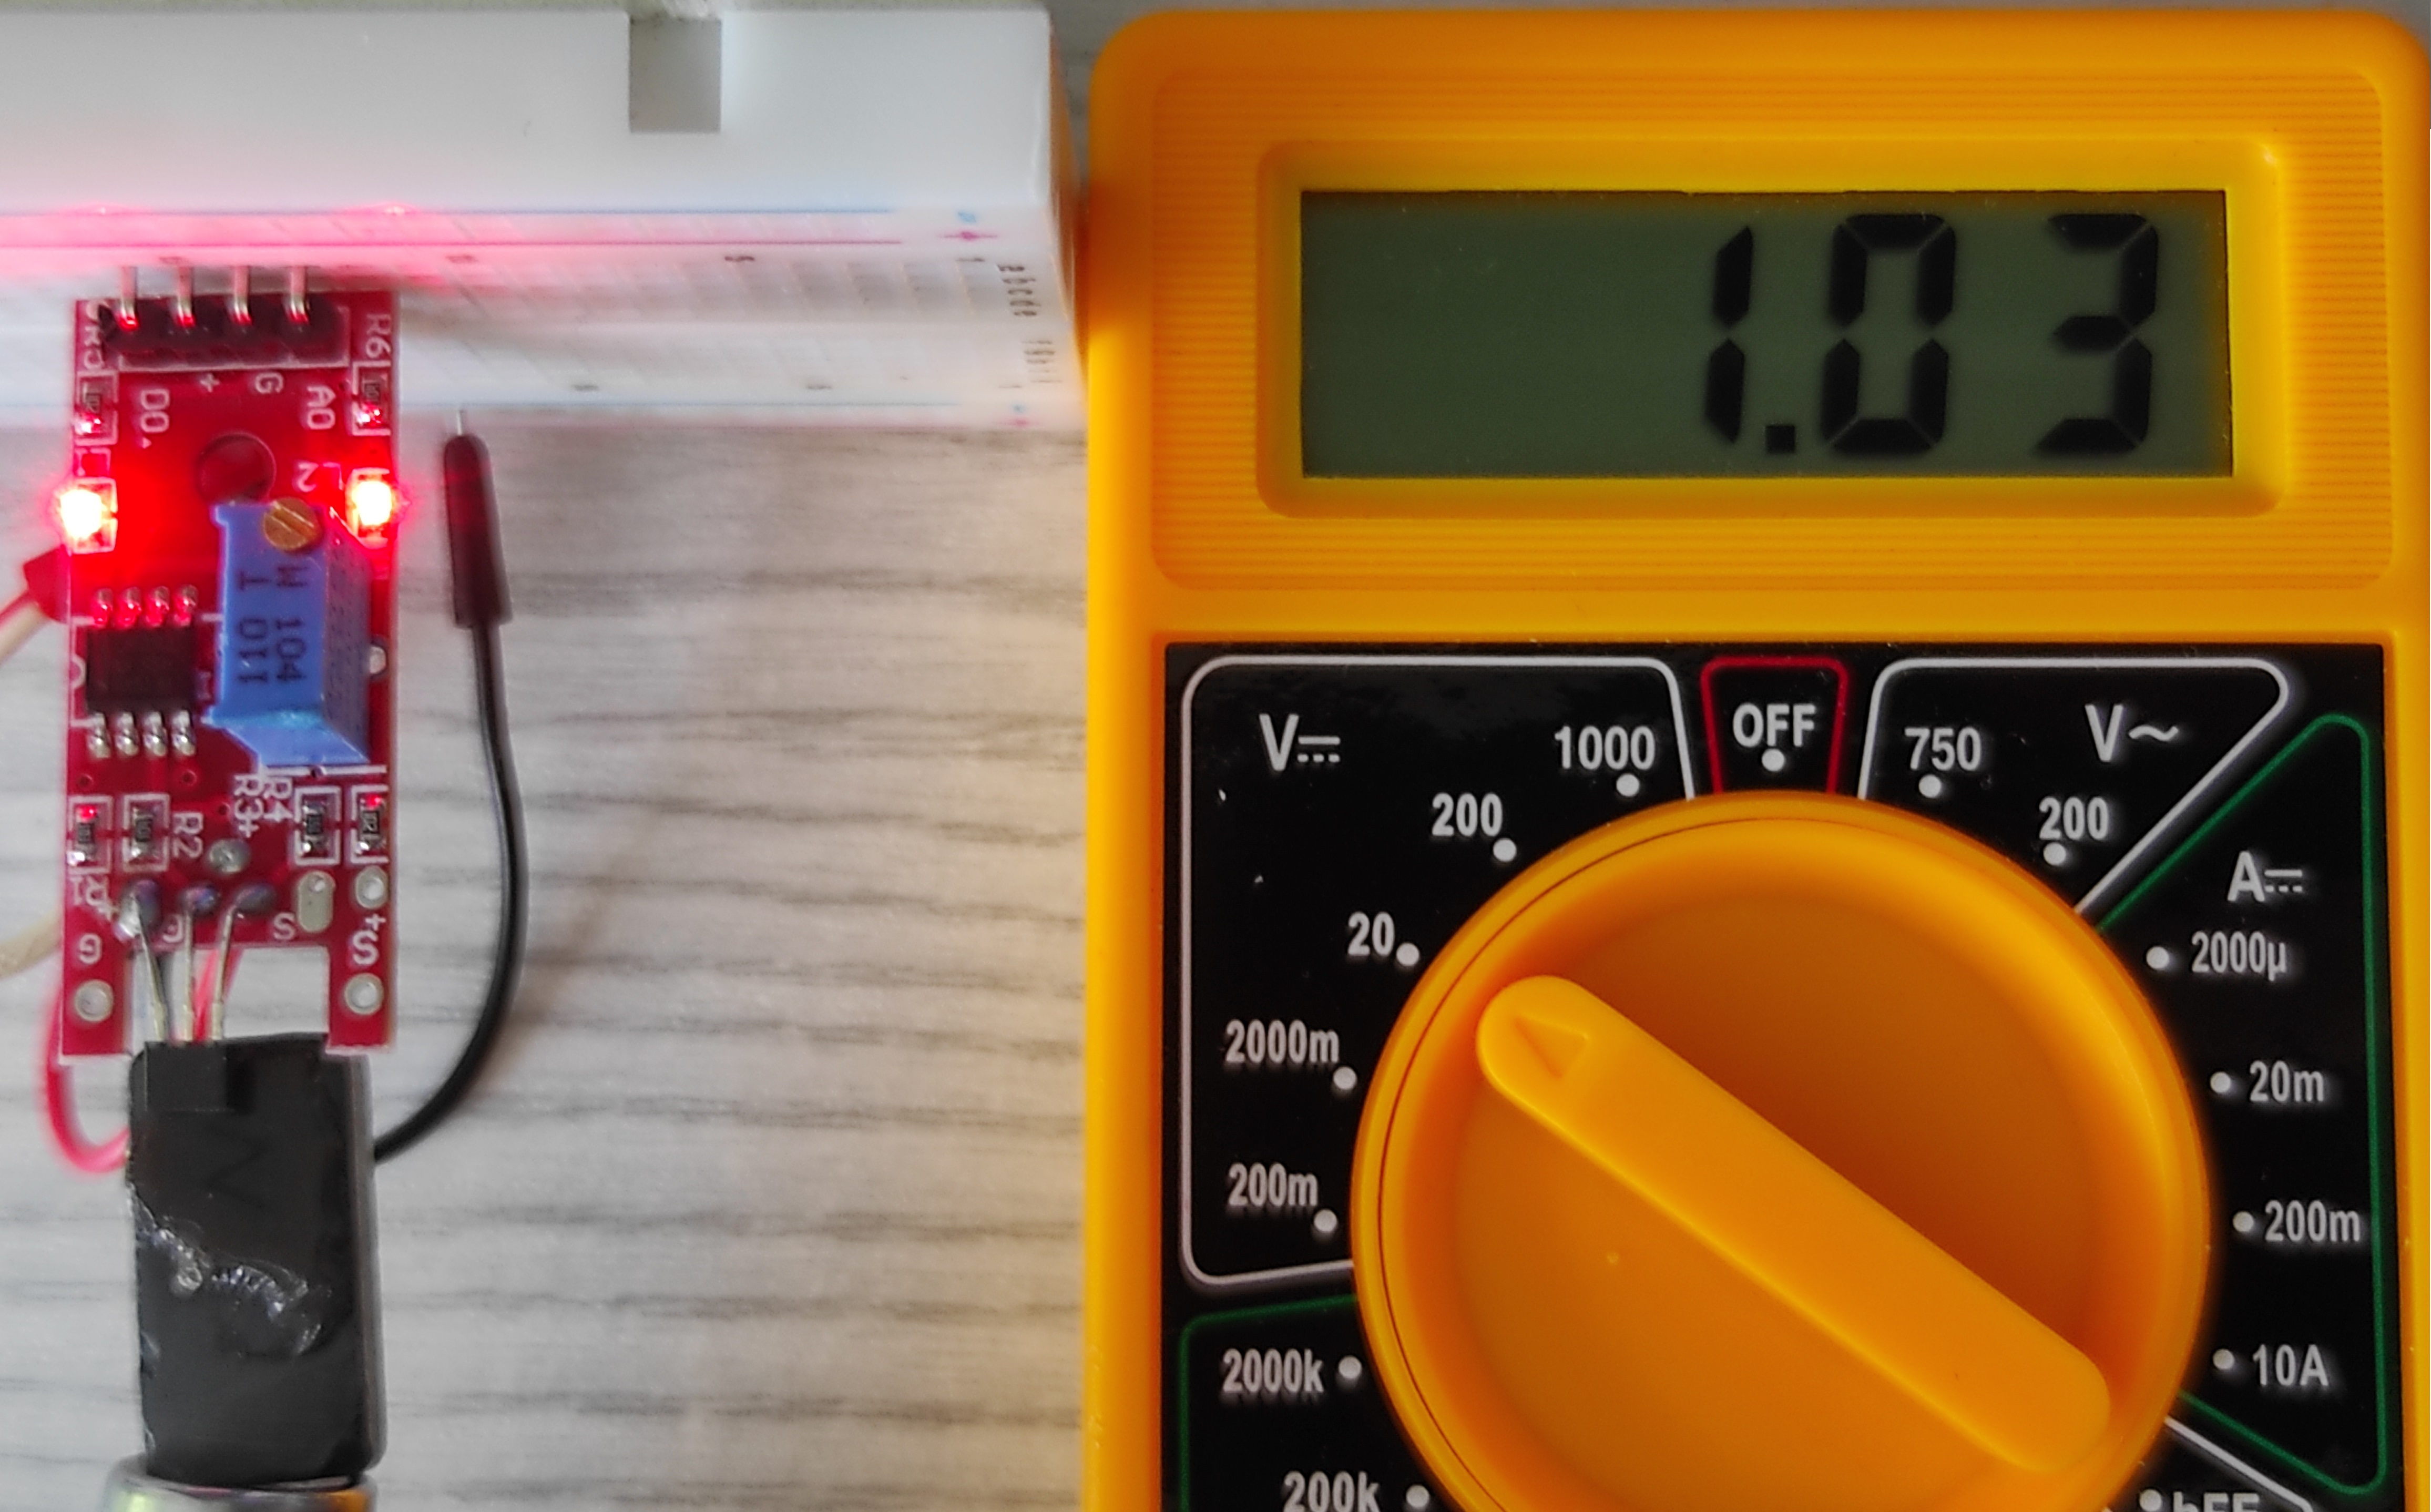
\includegraphics[width=.82\linewidth]{fig/KY-024/działanie_ukladu/analog_min.jpg}
\caption{Wykrycie bieguna N magnesu}
\label{fig:_analog_min_def_on}
\end{subfigure}%
%%%%%%%%%%%%%%%%%%%%%%%%%%%%%%%%%%%%%%%%%%%%%%%%%%%%%%%%%%%%%%%%%%%%%%%%%%%%%%%%%
\begin{subfigure}{.5\textwidth}
\centering
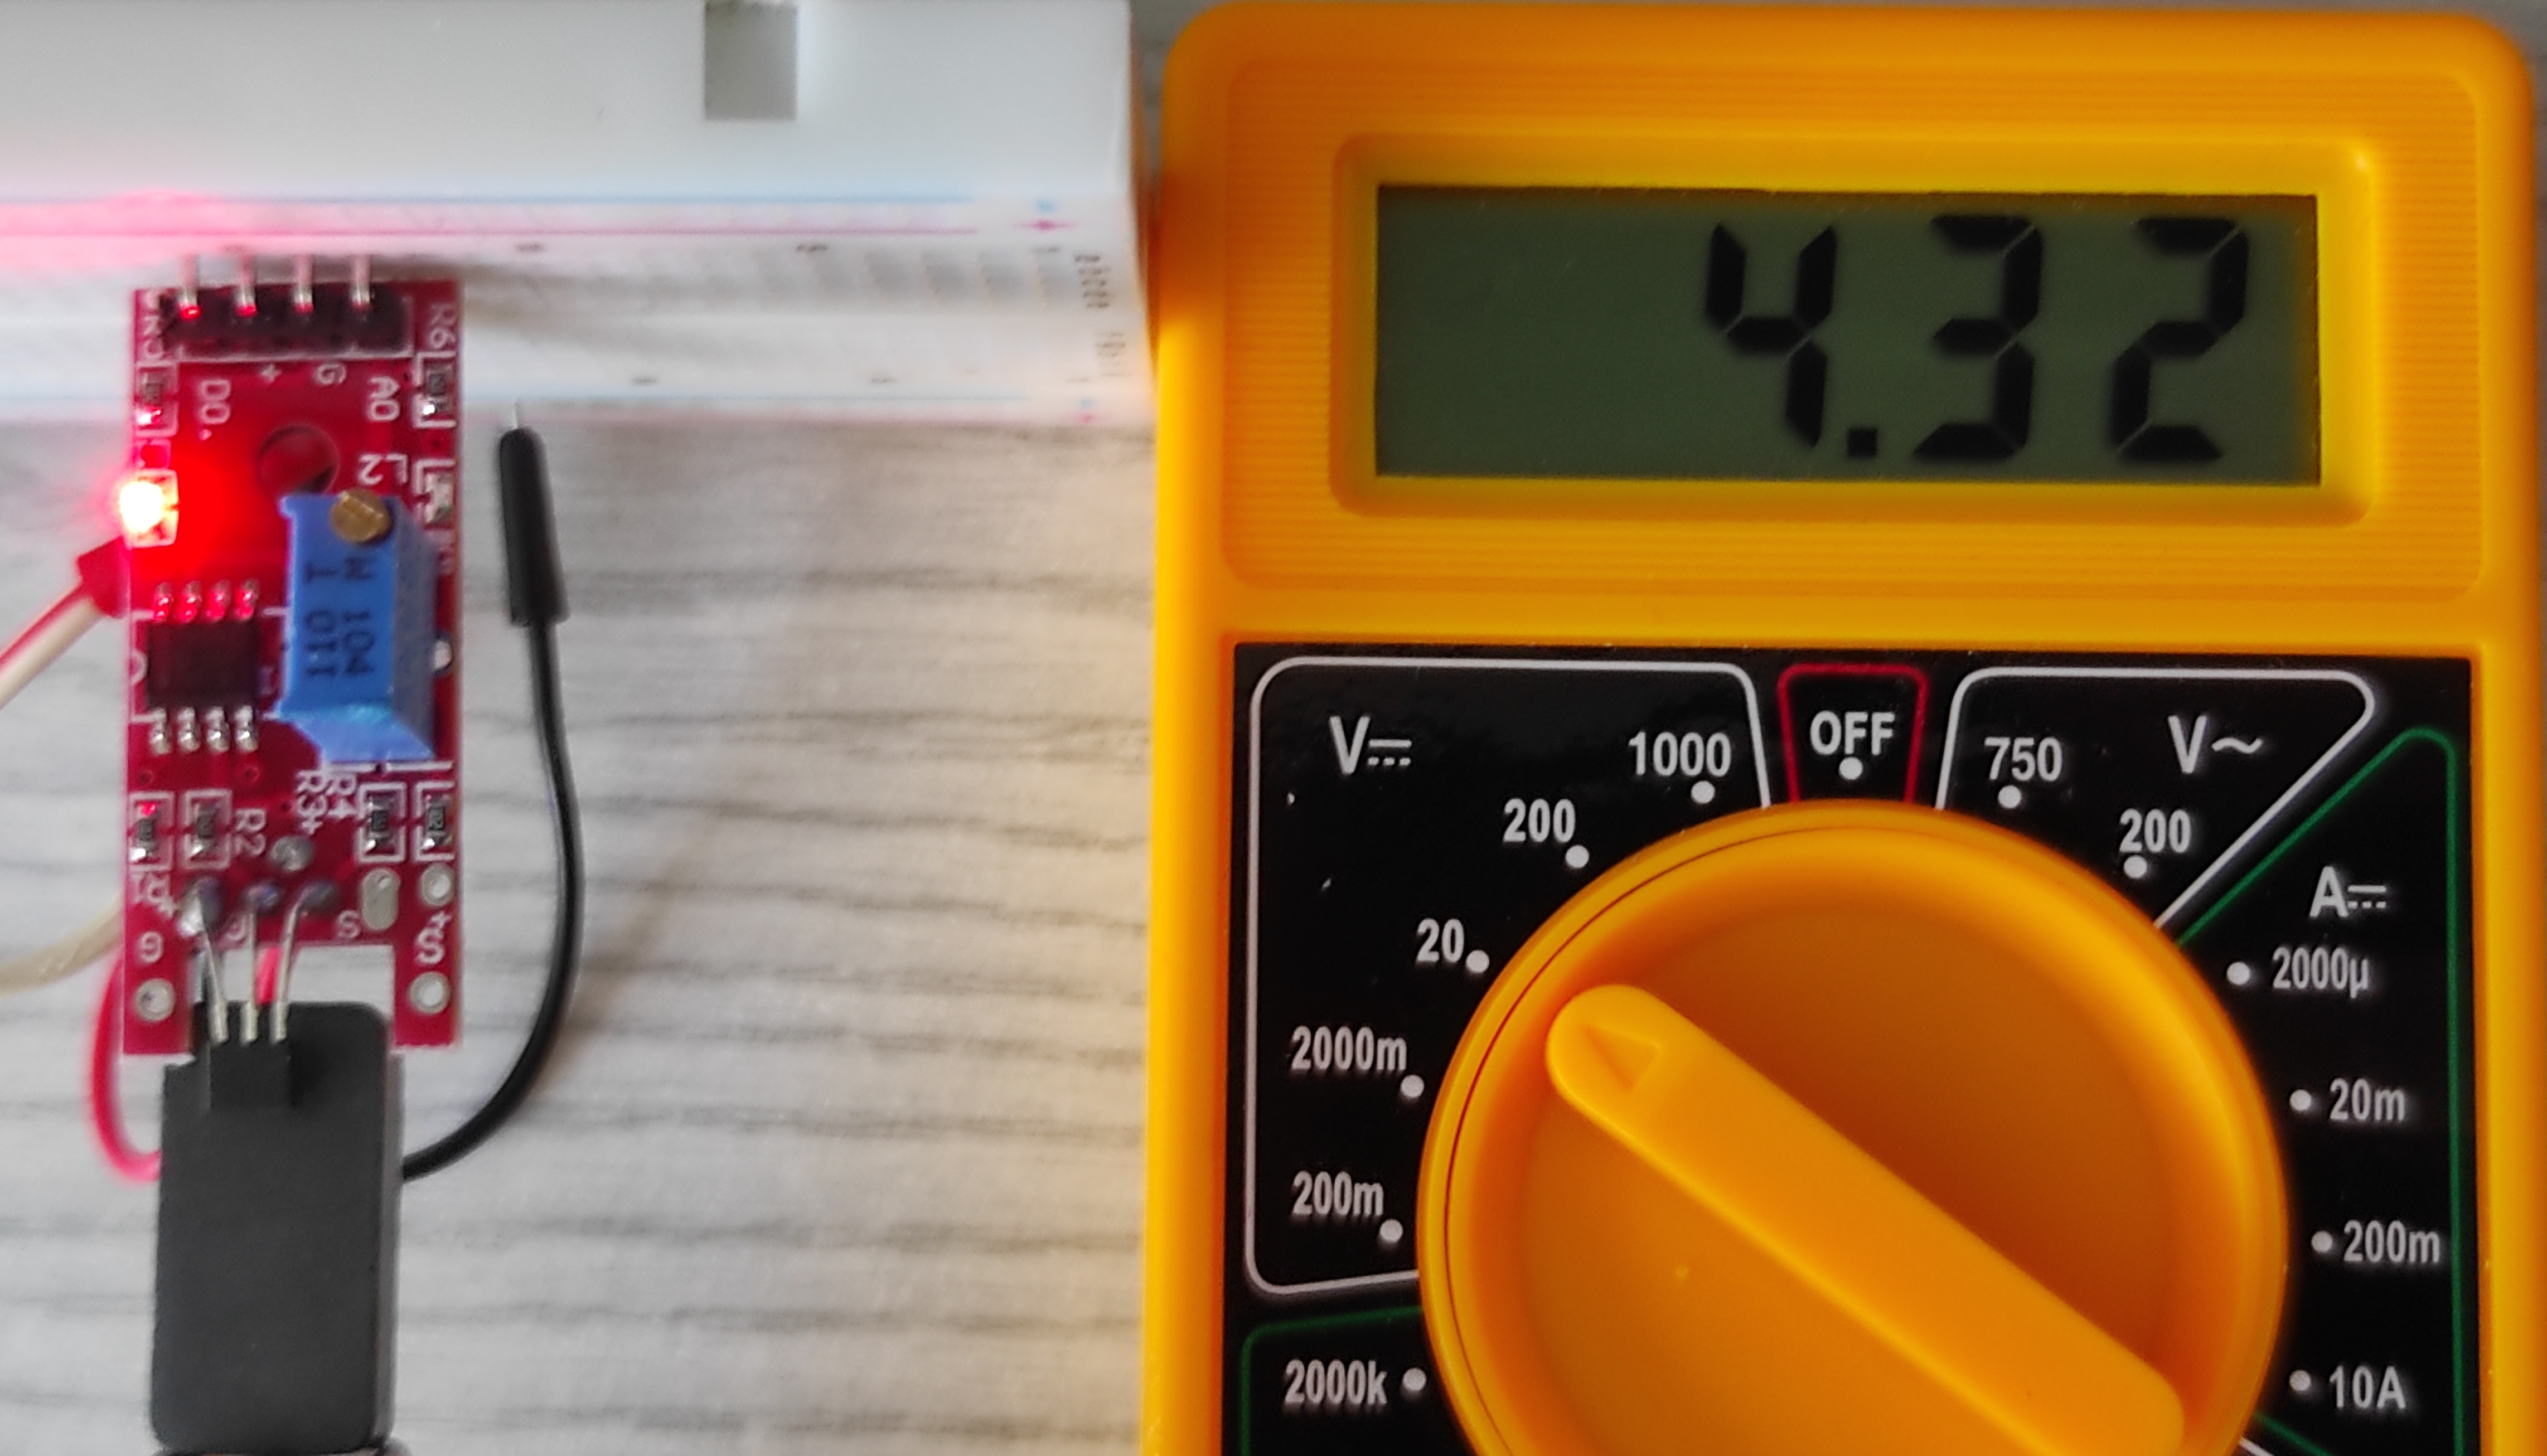
\includegraphics[width=.93\linewidth]{fig/KY-024/działanie_ukladu/analog_max.jpg}
\caption{Wykrycie bieguna S magnesu}
\label{fig:_analog_max_def_on}
\end{subfigure}
%%%%%%%%%%%%%%%%%%%%%%%%%%%%%%%%%%%%%%%%%%%%%%%%%%%%%%%%%%%%%%%%%%%%%%%%%%%%%%%%%
% \caption{PODPIS}
\label{fig:miernik3}
\end{figure}
%%%%%%%%%%%%%%%%%%%%%%%%%  TWO IMAGES SIDE BY SIDE  %%%%%%%%%%%%%%%%%%%%%%%%%%%%%

\begin{figure}[H]
    \centering
    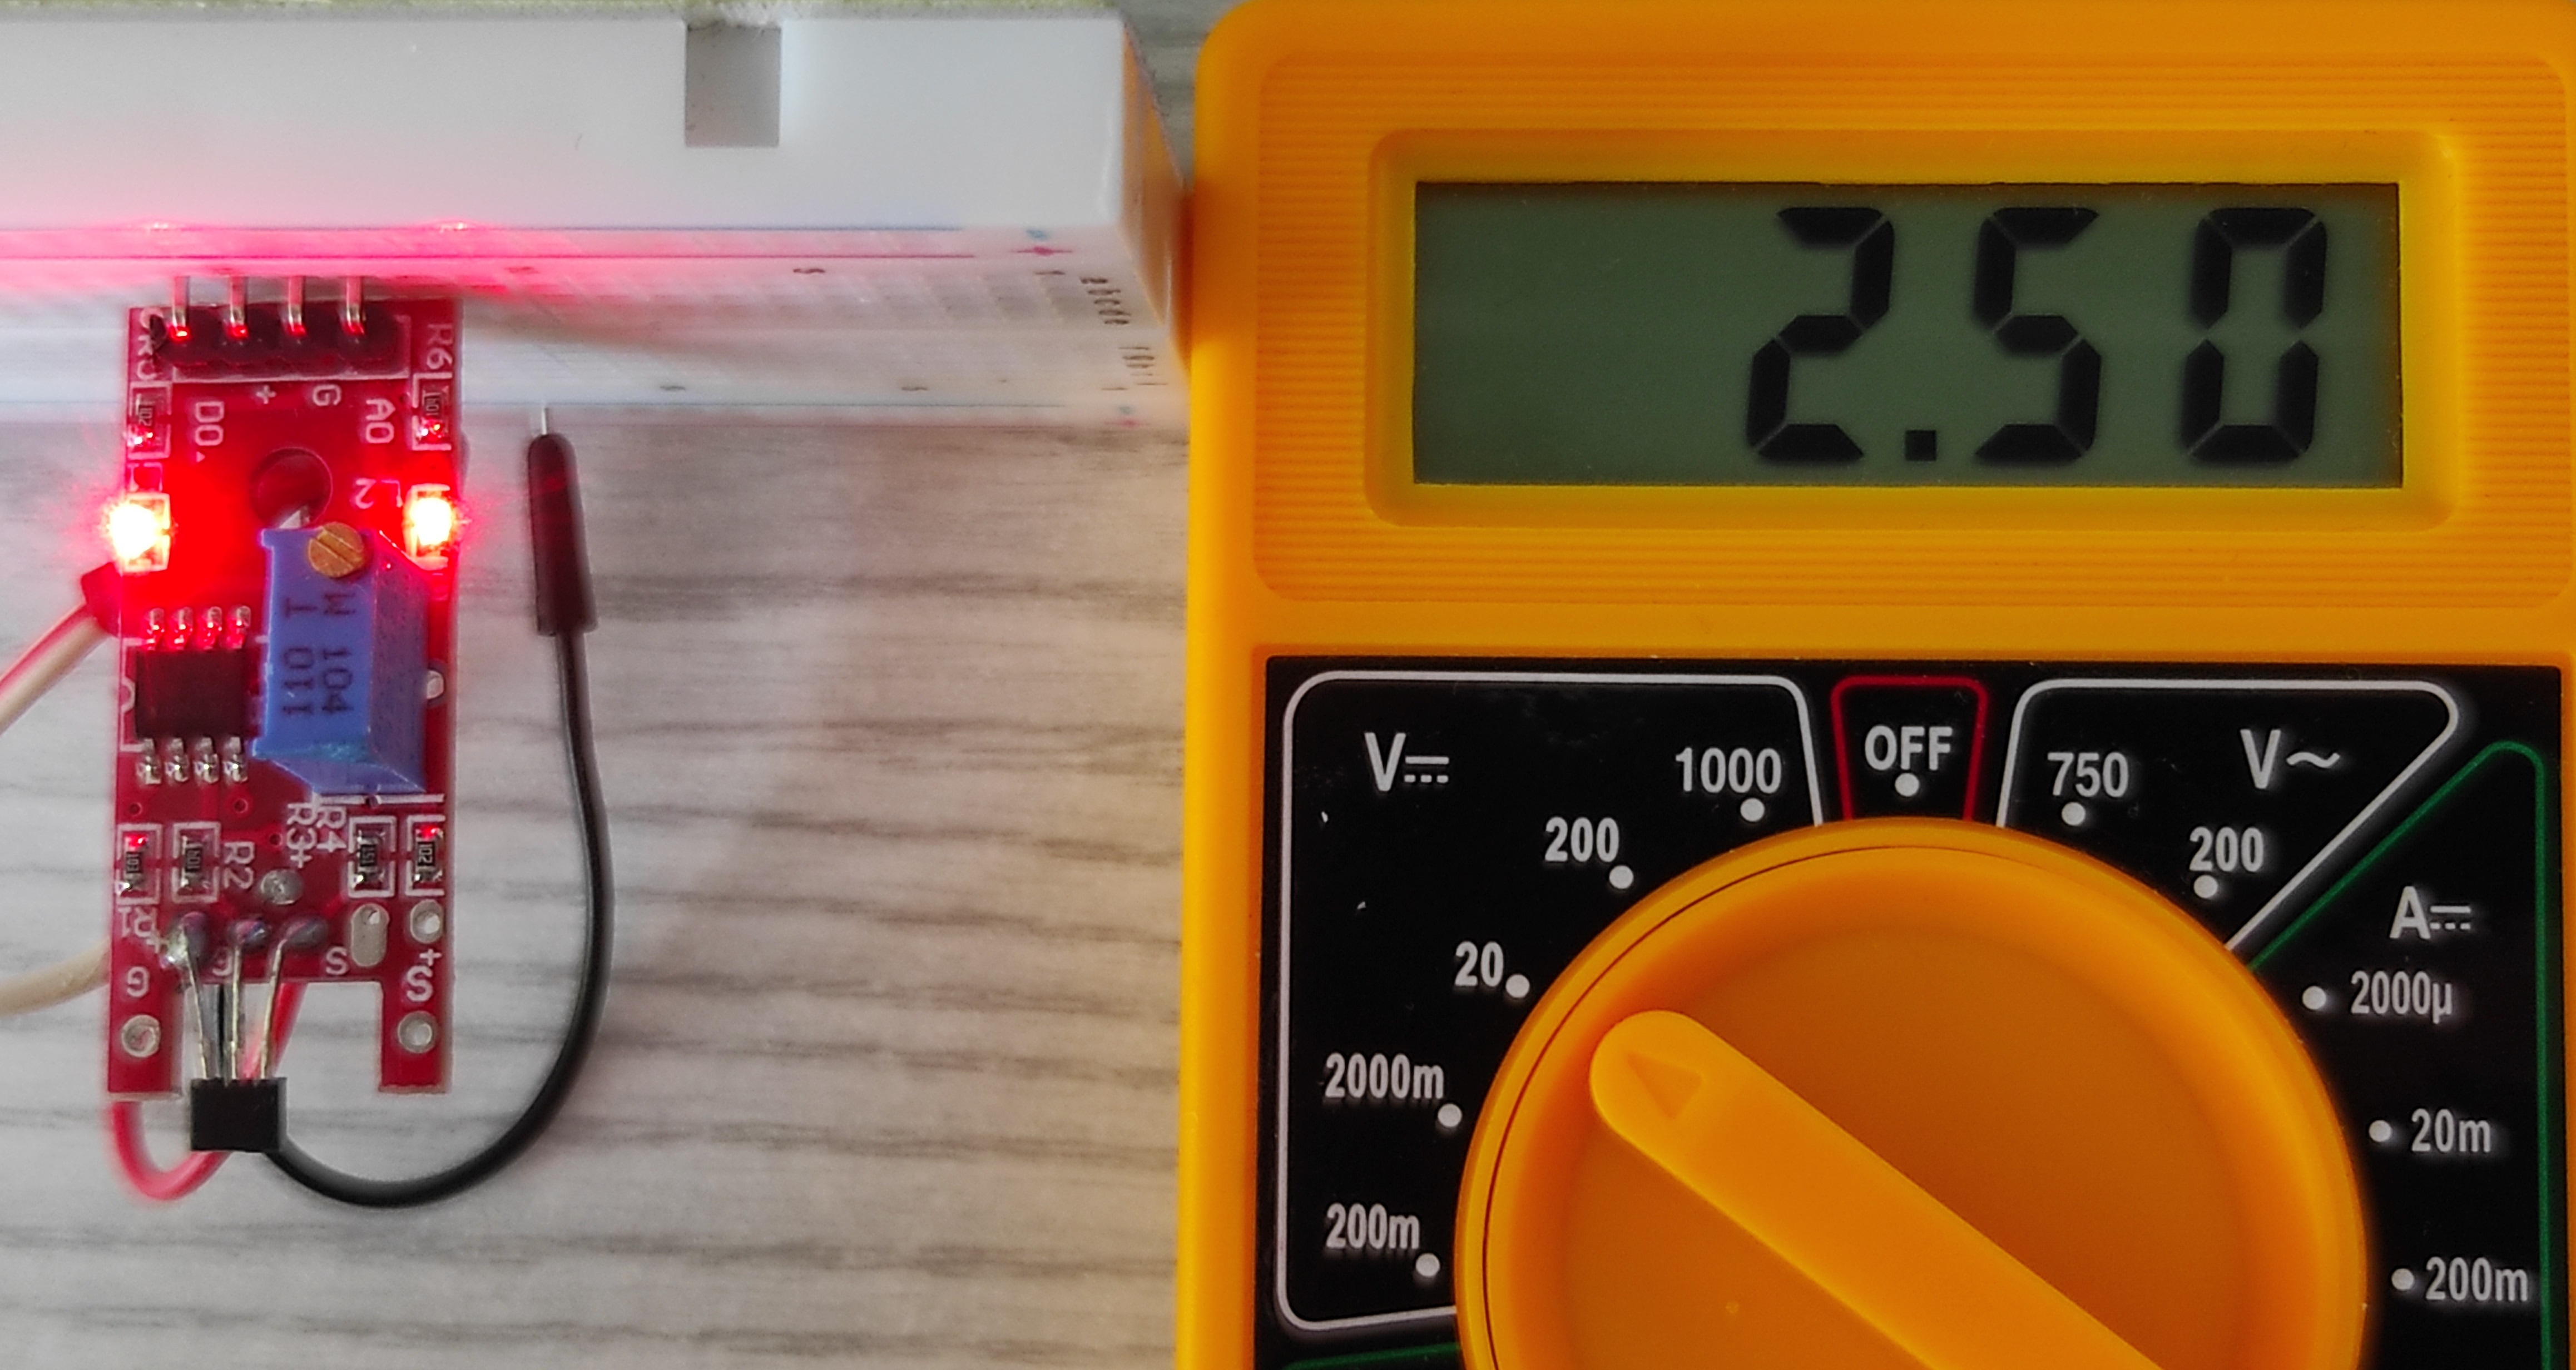
\includegraphics[width=.45\textwidth]{fig/KY-024/działanie_ukladu/analog_mid.jpg}
    \caption{Brak pola magnetycznego}
    \label{fig:_analog_mid_def_on}
\end{figure}
\end{itemize}

\newpage

W poniższym przykładzie użyto płytki rozwojowej STM32 NUCLEO-F767ZI. Układ połączeń przedstawiony na rysunku (\ref{fig:_polaczenie_ukladu}) oraz program dla płytki NUCLEO-F746ZG będzie identyczny. Do wykorzystania pełnej funkcjonalności czujnika wymagana jest konfiguracja dwóch pinów - jednego jako GPIO i drugiego jako ADC. Konfiguracja pliku \texttt{.IOC} i kod zawarte są w \texttt{Suplement \#2}.
\vspace{0.25cm}
\begin{figure}[H]
    \centering
    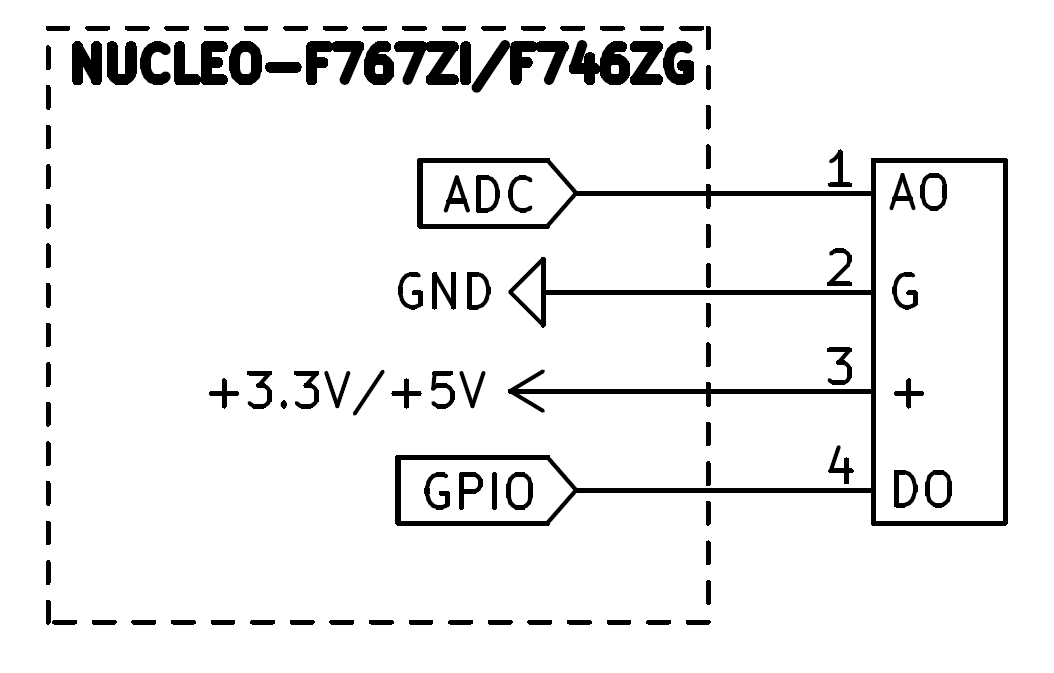
\includegraphics[width=0.6\textwidth]{fig/KY-024/polaczenie_modulu/polaczenie_nucleo.png}
    \caption{Połączenie układu z mikroprocesorem}
    \label{fig:_polaczenie_ukladu}
\end{figure}
\vspace{0.25cm}

Program skonfigurowano tak, aby po wykryciu pola magnetycznego włączana była zielona dioda LD1 znajdująca się na płytce NUCLEO. Poniżej przedstawiono zdjęcia fizycznego połączenia z mikrokontrolerem. Przewód koloru fioletowego przesyła sygnał analogowy, a koloru brązowego sygnał cyfrowy z czujnika.
% TUTAJ FOTY ODNOSNIE TEGO
%%%%%%%%%%%%%%%%%%%%%%%%%  TWO IMAGES SIDE BY SIDE  %%%%%%%%%%%%%%%%%%%%%%%%%%%%%
\vspace{0.25cm}
\begin{figure}[H]
\centering
%%%%%%%%%%%%%%%%%%%%%%%%%%%%%%%%%%%%%%%%%%%%%%%%%%%%%%%%%%%%%%%%%%%%%%%%%%%%%%%%%
\begin{subfigure}{.5\textwidth}
\centering
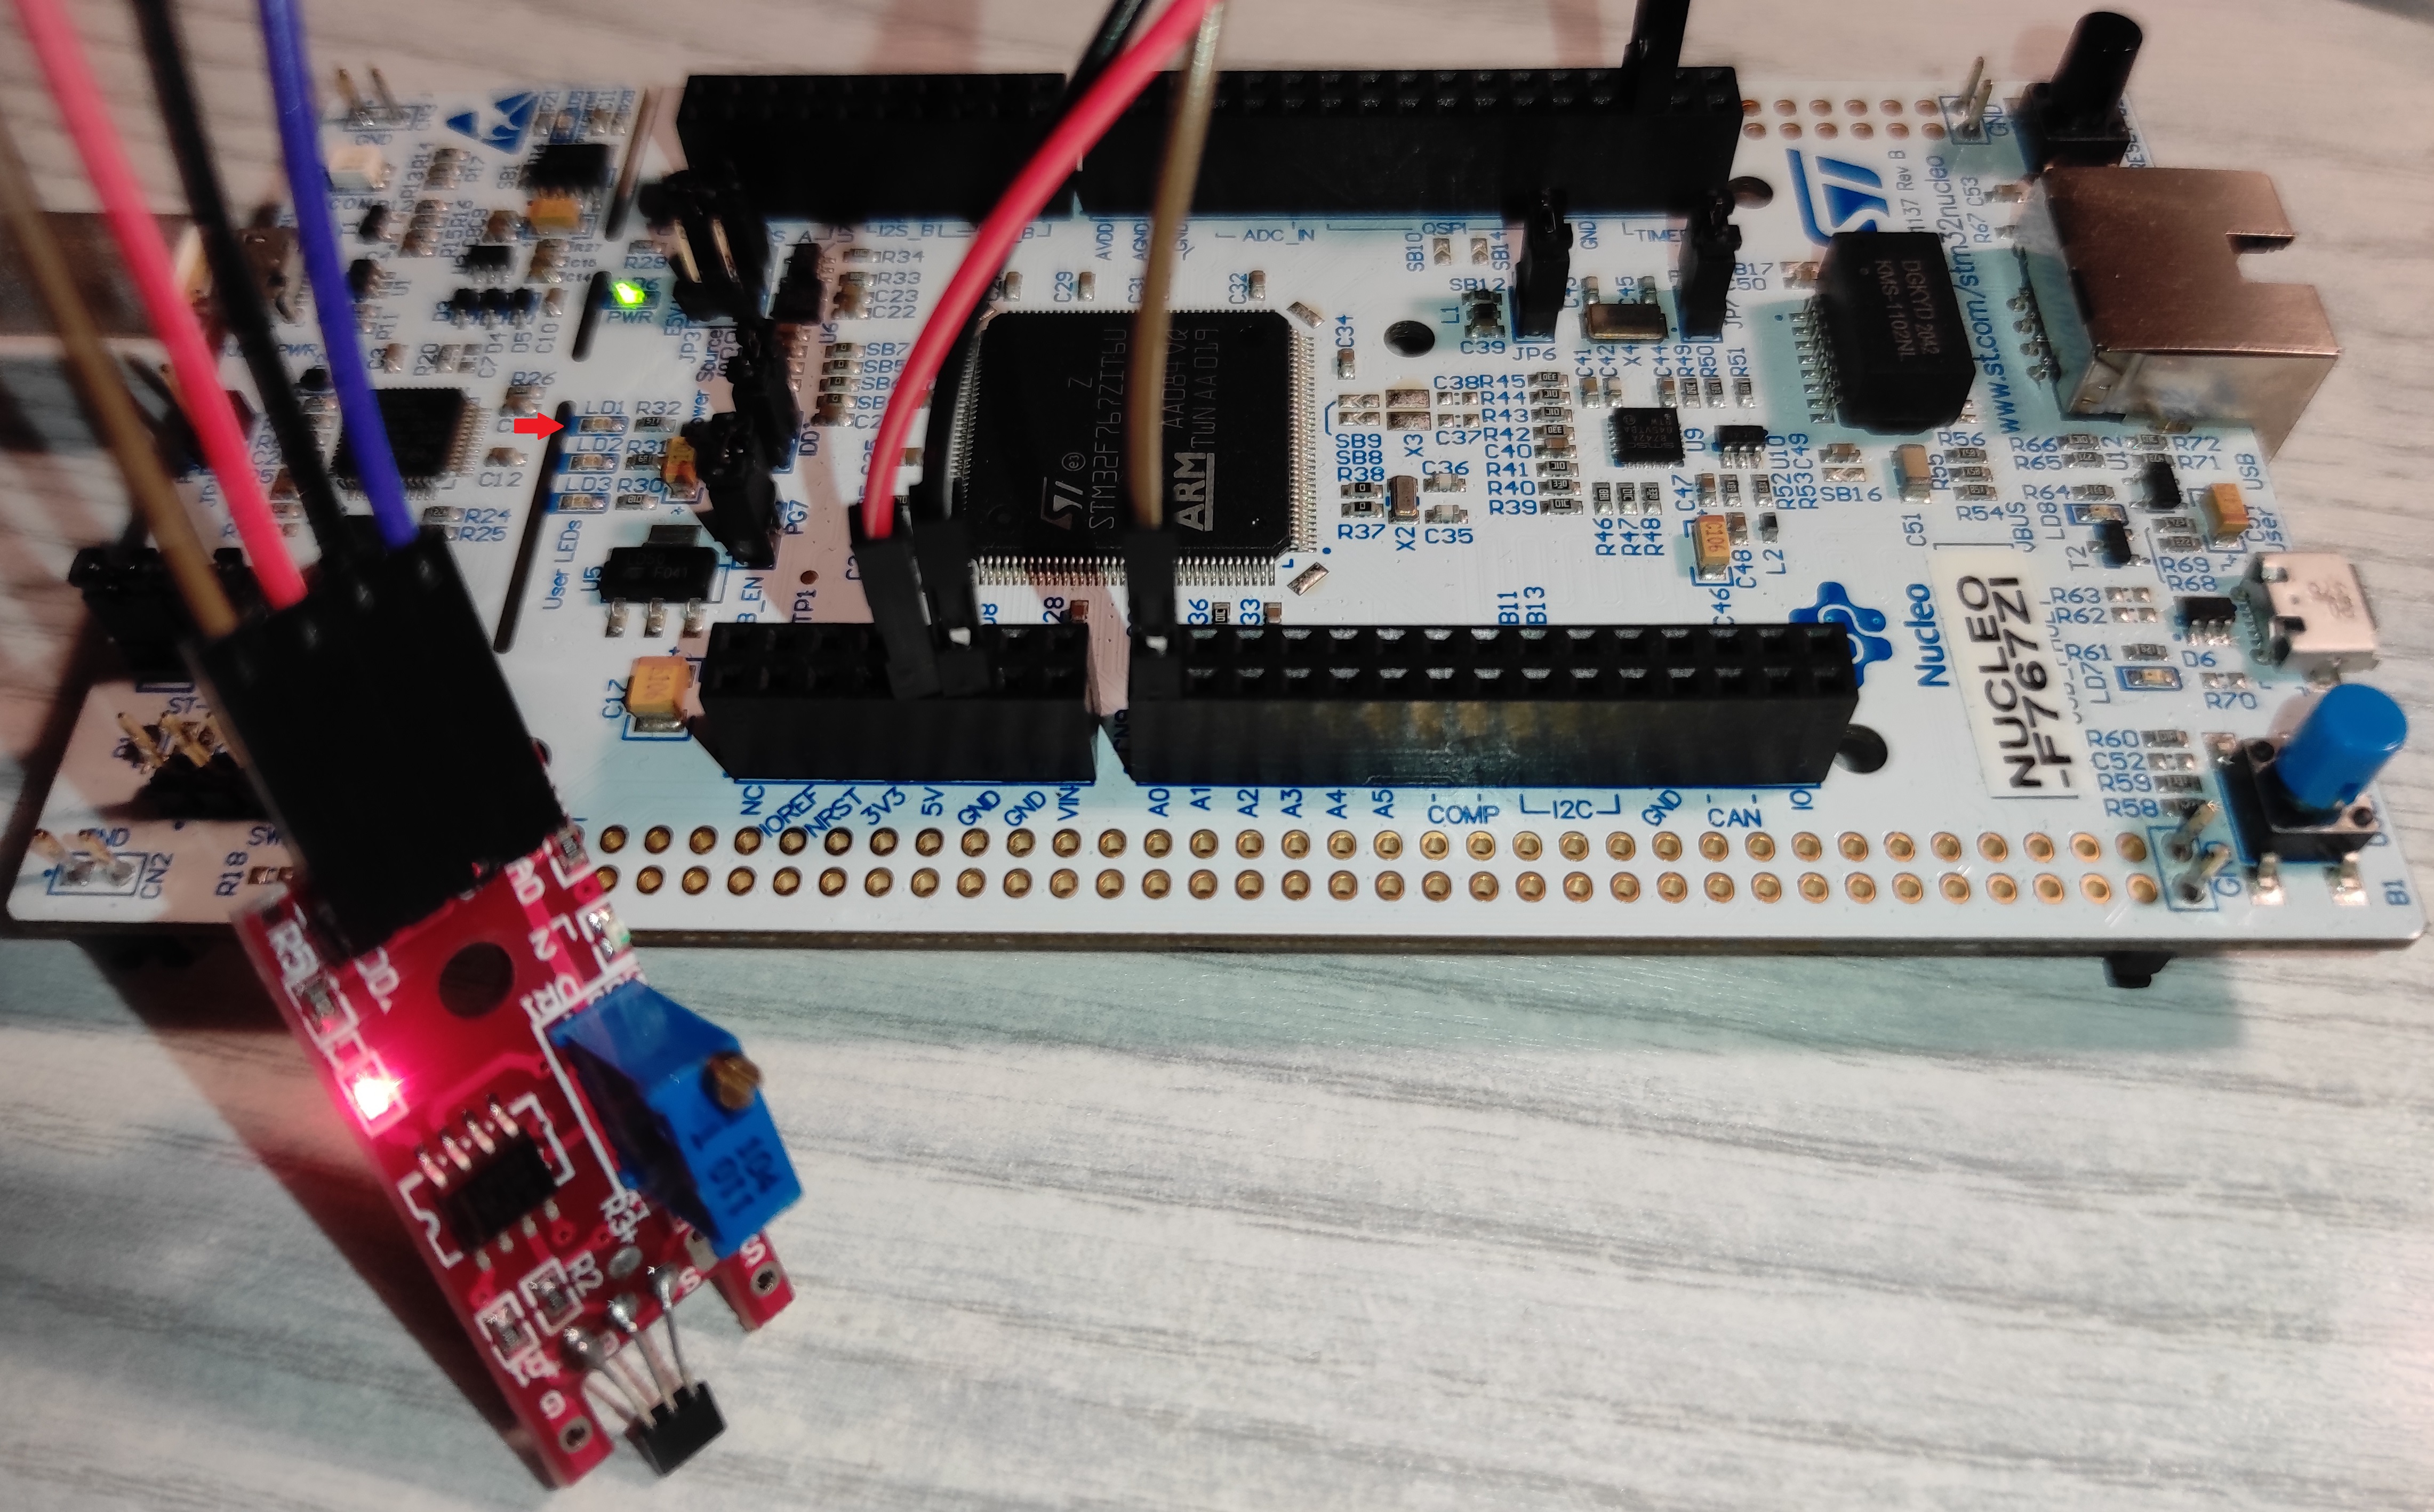
\includegraphics[width=.98\linewidth]{fig/KY-024/działanie_ukladu/zdj_off.jpg}
\caption{Brak pola magnetycznego}
\label{fig:_uklad_off}
\end{subfigure}%
%%%%%%%%%%%%%%%%%%%%%%%%%%%%%%%%%%%%%%%%%%%%%%%%%%%%%%%%%%%%%%%%%%%%%%%%%%%%%%%%%
\begin{subfigure}{.5\textwidth}
\centering
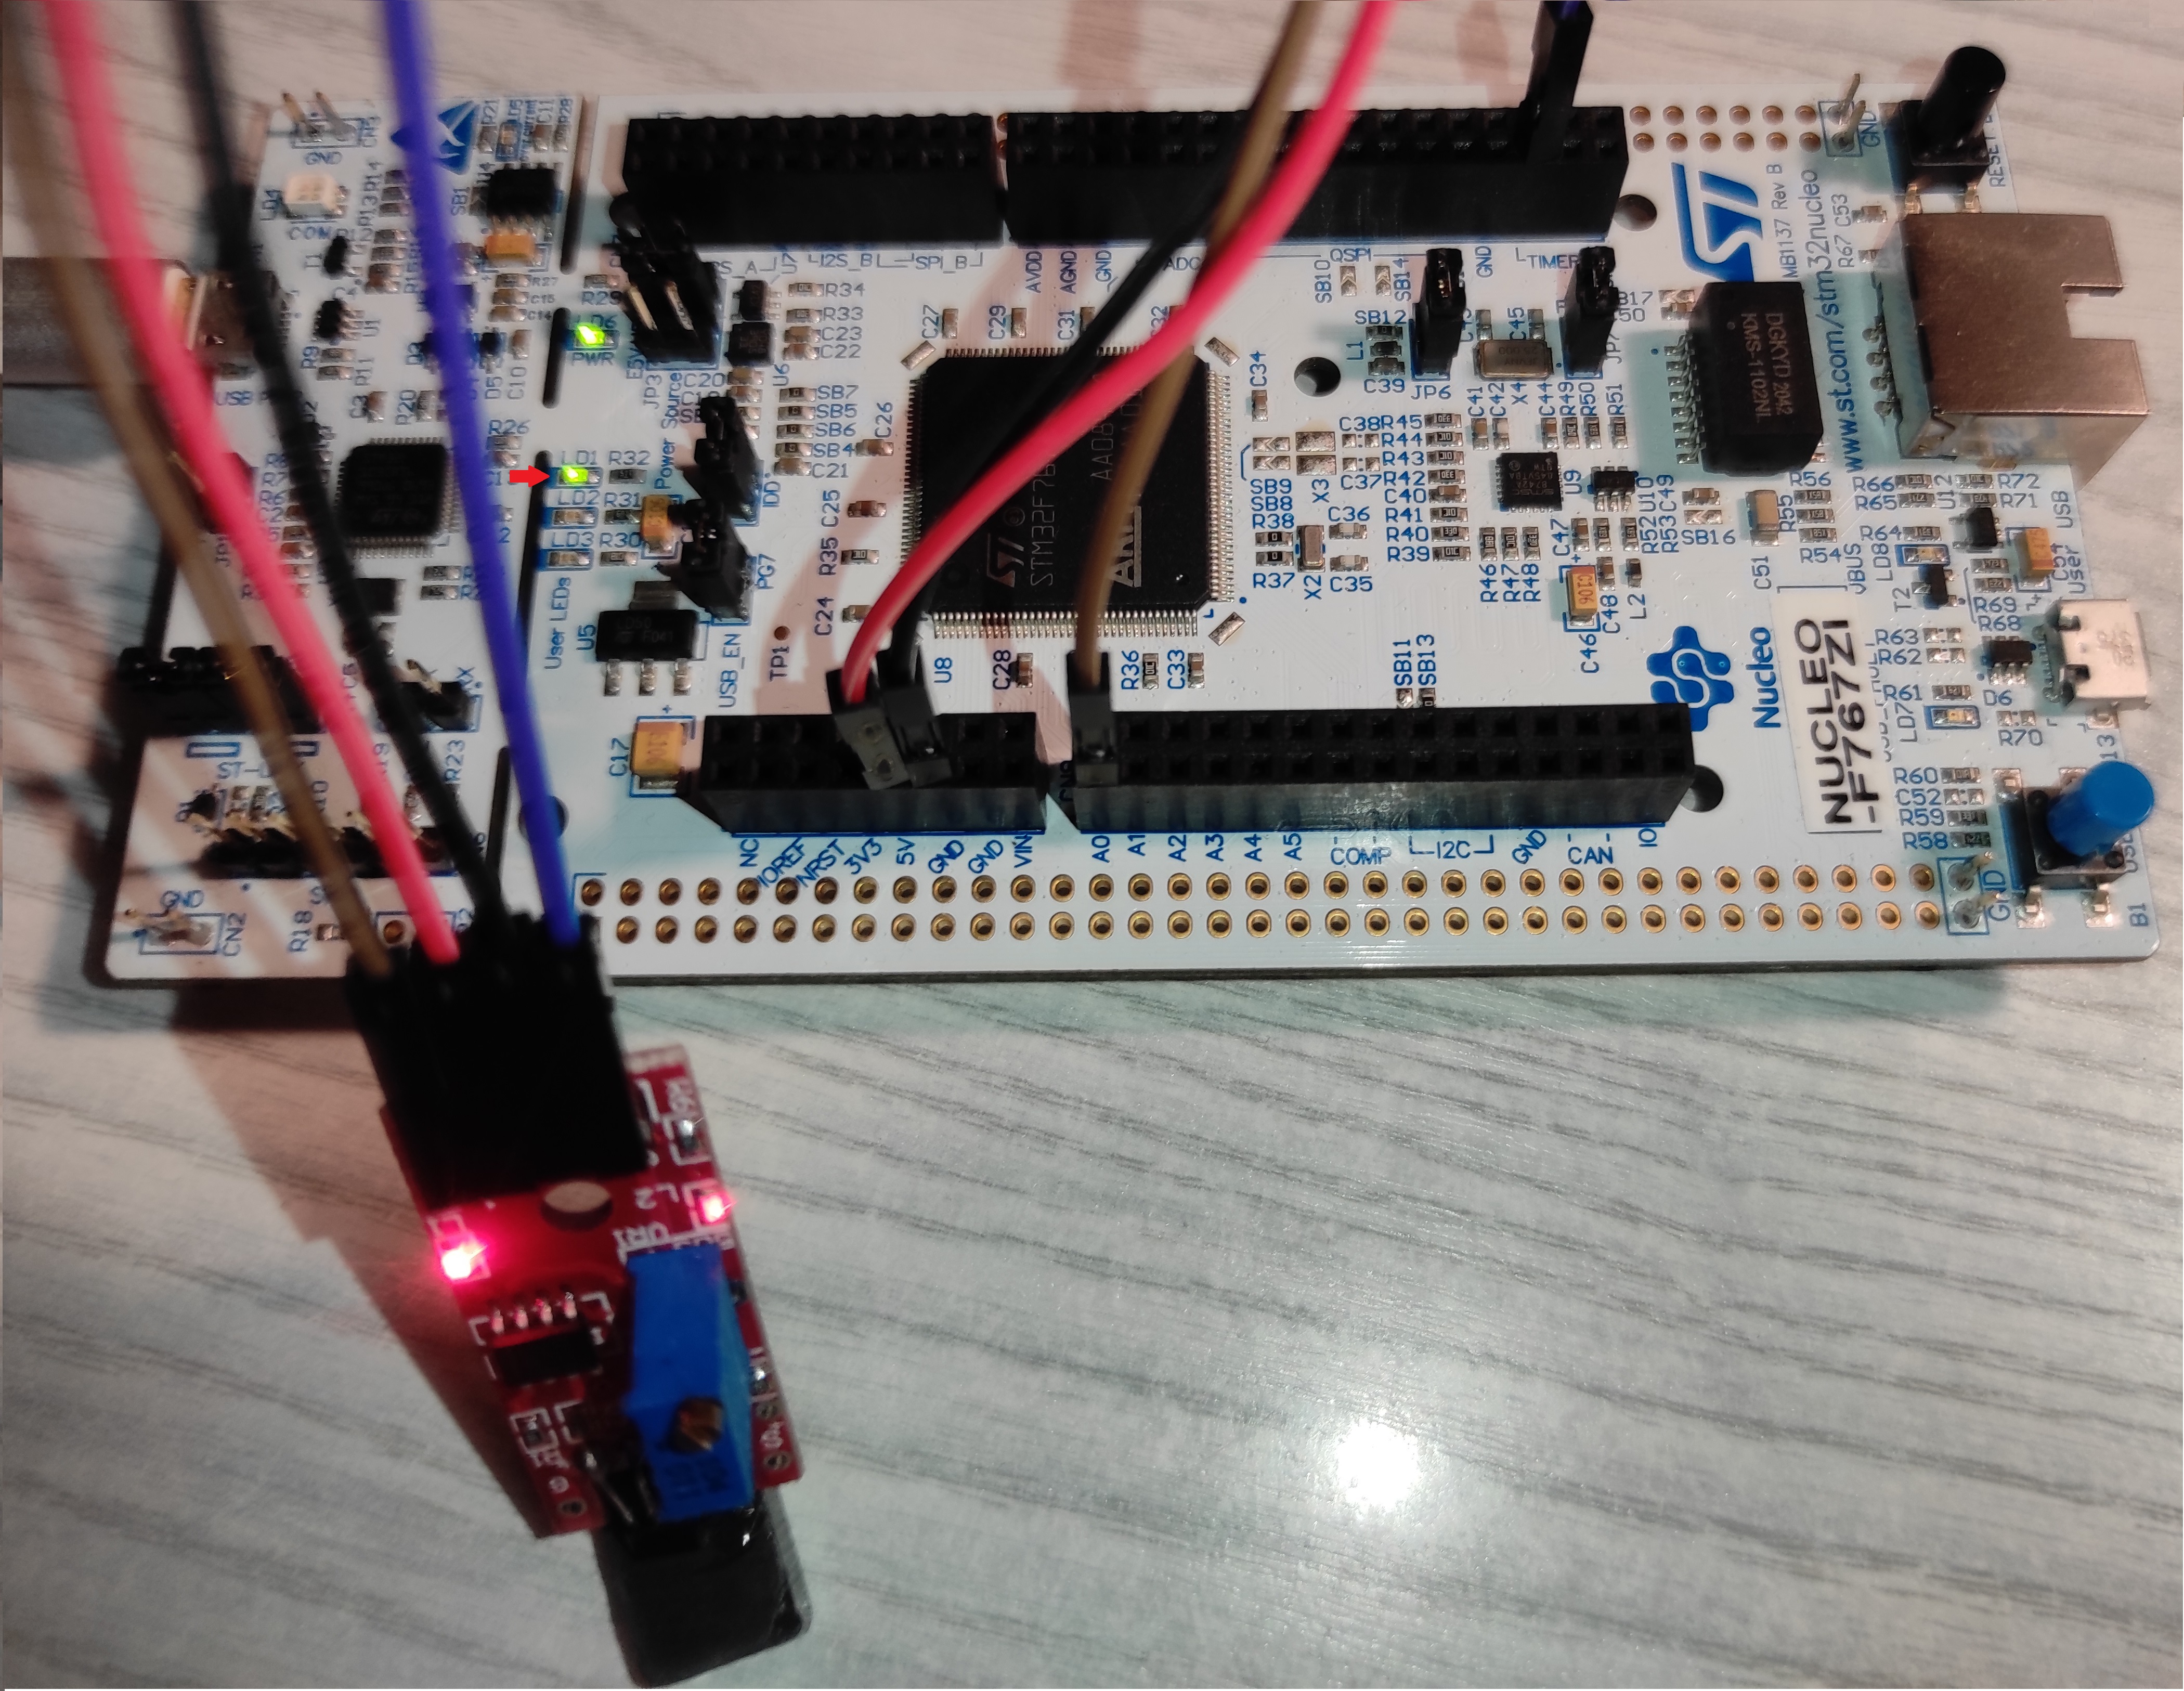
\includegraphics[width=.8\linewidth]{fig/KY-024/działanie_ukladu/zdj_on.jpg}
\caption{Pole magnetyczne wykryte}
\label{fig:_uklad_on}
\end{subfigure}
%%%%%%%%%%%%%%%%%%%%%%%%%%%%%%%%%%%%%%%%%%%%%%%%%%%%%%%%%%%%%%%%%%%%%%%%%%%%%%%%%
% \caption{PODPIS}
\label{fig:mikroproc}
\end{figure}
\vspace{0.25cm}
%%%%%%%%%%%%%%%%%%%%%%%%%  TWO IMAGES SIDE BY SIDE  %%%%%%%%%%%%%%%%%%%%%%%%%%%%%
Działanie układu z użyciem wyjścia analogowego AO dla lepszego zobrazowania przedstawiono na załączonym w \texttt{Suplement Wideo} materiale wideo.

\newpage
\printbibliography[heading=bibintoc]

\end{document}